\documentclass[a4paper,ngerman,oneside]{scrbook}
\usepackage[ngerman]{babel}
\usepackage[autostyle=true,german=quotes]{csquotes}
\usepackage[utf8]{inputenc}
\usepackage[T1]{fontenc}
\usepackage{xspace}

\usepackage{hyperref}
\usepackage{cleveref}

\usepackage{scrhack}

\usepackage{enumitem}
\setlist[itemize]{noitemsep, topsep=0pt}

\usepackage{graphicx,tabularx}
\usepackage{textcomp}
\usepackage{xcolor}
\usepackage{subcaption}
\usepackage[color]{changebar}
\setlength\changebarsep{10pt}


\newcommand{\nach}{\xspace\textrightarrow\xspace}
\newcommand{\cmnd}[1]{\texttt{#1}\xspace}

\newcommand{\EPL}{\textsf{EPL}\xspace}
\newcommand{\Einsatz}{\textsf{Einsatzplaner}\xspace}
\newcommand{\Personal}{\textsf{Personalplaner}\xspace}
\newcommand{\datei}[1]{\texttt{#1}\xspace}
\newcommand{\aktion}[1]{\enquote{#1}\xspace}
\newcommand{\button}[1]{\enquote{#1}\xspace}

\let\bslash\textbackslash


\newenvironment{neu}{ \color{red} \changebar }{ \endchangebar }
\newenvironment{hinweis}{ \medskip \noindent\textsf{\textbf{Hinweis\ }} } {\medskip}

\graphicspath{{./img/}}

\titlehead{}

\subject{\centering
\includegraphics[width=0.25\textwidth]{../../Icon/EPL.png}}
\title{Anleitung EPL-Programmpaket}
\subtitle{Version 1.8.3}
\author{Philipp Schepper}
\date{Stand: \today}
%\publishers{\Huge{\textsf{Arbeitsdatei}}}

\begin{document}
\maketitle

\frontmatter
\tableofcontents
\chapter{Änderungshistorie}
\begin{tabularx}{\textwidth}{l|X}
  Datum & Änderung \\
  \hline
  \hline
  02.05.2020 &
    Dokument für Version 1.6 komplett neu herausgegeben.\newline
    Wichtige Informationen zur Aktualisierung von Version 1.5 auf 1.6 in \cref{epl:update:1.5-1.6}.\\
  \hline
  06.08.2020 &
    Version 1.6.1 eingefügt.\newline
    Veränderungen hauptsächlich in \cref{einsatz:personal}.
    Ansonsten überwiegend Fehlerbehebungen.
    \\
  \hline
  16.10.2020 &
    Version 1.6.2 eingefügt.\newline
    \cref{epl:allg:datei:schreibschutz} eingefügt.\newline
    Beachten Sie die Hinwiese zur Installation in \cref{epl:allg:installation}.
    \\
  \hline
  02.04.2021 &
    Version 1.7.0 eingefügt.\newline
    Dokumentation überarbeitet, da das Programm in \Einsatz und \Personal aufgeteilt wurde.
    \\
  \hline
  13.06.2021 &
    Version 1.7.1 eingefügt.\newline
    Kleinere Korrekturen.
    \\
  \hline
  13.08.2021 &
    Version 1.8:\newline
    Beiträge eingeführt (\cref{personal:mitglieder:beitrag}).
    \\
  \hline
  17.08.2021 &
    Version 1.8.1: Fehlerbehebungen.
\end{tabularx}
Änderungen seit Version 1.7.1 sind farblich hervorgehoben.


\mainmatter

\part{EPL-Programmfamilie}
\chapter{Allgemeines}\label{epl:allg}
Das EPL-Programmpaket dient dazu die Verwaltungstätigkeiten einer Museumseisenbahn zu verbessern.
Dazu können mit dem Programm \Einsatz Fahrtage und Arbeitseinsätze verwalten werden,
sowie die Einsatzzeiten der Mitglieder erfasst und berechnet werden.
Fahrtage unterschieden sich von Arbeitseinsätzen dadurch, dass das Personal direkt bestimmten Aufgabengebieten zugeordnet werden kann.
Ebenso können Reservierungen eingetragen werden.
Mit dem Programm \Personal kann eine Verwaltung der Mitglieder und Speicherung der entsprechenden Daten durchgeführt werden.

\begin{figure}[h]
  \centering
  \begin{subfigure}{0.3\textwidth}
    
\includegraphics[width=\textwidth]{../../Icon/EPL.png}
    \caption{Logo von \EPL}
  \end{subfigure}

  \begin{subfigure}{0.3\textwidth}
    
\includegraphics[width=\textwidth]{../../Icon/Einsatzplaner.png}
    \caption{Logo des \Einsatz}
  \end{subfigure}
  \begin{subfigure}{0.3\textwidth}
    
\includegraphics[width=\textwidth]{../../Icon/Personalplaner.png}
    \caption{Logo des \Personal}
  \end{subfigure}
  \caption{Die Logos des Programmpakets}
\end{figure}


\section{Die EPL-Datei}\label{epl:allg:datei}
Die Daten der Programme werden in einer gemeinsamen Datei mit der Endung \datei{.ako} gespeichert.
In ihr sind alle Personaldaten und alle Daten zu den Aktivitäten gespeichert.
Sowohl \Personal als auch \Einsatz können somit auf den gleichen Datenbestand zurückgreifen.

\subsection{Schreibschutz}\label{epl:allg:datei:schreibschutz}
Beim Öffnen einer Datei \datei{X.ako} wird automatisch eine neue Datei mit dem Namen \datei{X.ako.lock} erstellt.
Durch diese Datei wird sichergestellt, dass nicht mehrere Personen gleichzeitig an der Datei \datei{X.ako} arbeiten.
Wird eine bereits geöffnete Datei erneut geöffnet (vom gleichen oder fremden Benutzer),
kann sie nur schreibgeschützt geöffnet werden und Änderungen können nicht gespeichert werden.
Beim Schließen einer Datei bzw.\ beim Beenden des Programms wird die Datei \datei{X.ako.lock} automatisch wieder gelöscht.
Danach kann ein anderer Benutzer die Datei \datei{X.ako} wieder uneingeschränkt öffnen.

\begin{hinweis}
  Der Schreibschutz steht nur effektiv zur Verfügung, wenn alle Beteiligten Version 1.6.2 oder neuer des Einsatzplaners verwendet.
  Wird eine frühere Version verwendet, kann die Datei allerdings weiterhin uneingeschränkt geöffnet und bearbeitet werden!
\end{hinweis}


\begin{hinweis}
  Die oben beschriebene Datei sollte unter normalen Umständen nicht manuell gelöscht werden, da dies zu Datenverlusten führen kann.
  Löschen Sie die Datei nur, wenn Sie sicherstellen können, dass keine weiteren Benutzer auf die Datei zugreifen.
\end{hinweis}


\subsection{Passwort-Schutz}\label{epl:allg:datei:passwort}
Es besteht die Möglichkeit die EPL-Datei mit einem Passwort-Schutz zu speichern.
Durch diesen können nur berechtigte Personen auf die Daten zugreifen.
Die Datei wird in diesem Fall verschlüsselt gespeichert.

\paragraph{Schutz einrichten und aufheben}
Der Schutz kann über den Eintrag \aktion{Eigenschaften} im Menü \aktion{Datei} geändert werden (Siehe auch \cref{fig:einsatz:kalender:upload}).
Das bisherige Passwort eingeben (sofern vorhanden) und das neue Passwort zweimal eingeben, um Tippfehler zu vermeiden.
Dann über den Knopf \button{Passwort ändern} die Änderung vornehmen.
Um einen vorhandenen Passwortschutz zu entfernen,
die beiden Felder für das neue Passwort frei lassen und mit dem Knopf bestätigen.


\begin{hinweis}
  Ohne das Passwort kann die Datei nicht mehr geöffnet werden und die Daten sind verloren.
  Stellen Sie deshalb sicher,
  dass Sie sich das Passwort merken können oder speichern es in einem Passwort-Manager.
\end{hinweis}


\section{Installation}\label{epl:allg:installation}
\subsection{macOS}
Laden Sie die bereitgestellte Datei herunter und entpacken Sie die \datei{.dmg}-Datei durch einen Doppelklick.
Ziehen Sie den Ordner \datei{EPL} zum Installieren in Ihren Programmordner.
Alternativ können Sie die beiden Programm im Ordner \datei{EPL} auch einzeln in den Programmordner Ihres Systems bewegen.

\subsection{Windows}
\begin{itemize}
  \item Laden Sie den Installer für Windows herunter.
  Öffnen Sie das Programm, und folgen dem Installationsprogramm.
  \item Merken Sie sich den Pfad, an dem Sie den Einsatzplaner installieren, z.B.\ \datei{C:{\bslash}Program Files (x86){\bslash}Einsatzplaner}.
  \item Wenn Sie den Einsatzplaner das erste Mal installieren,
  bzw.\ beim Start eine Fehlermeldung erhalten,
  navigieren Sie zu dem notierten Ordner.
  \item Dort finden Sie eine Datei \datei{vc\_redist.x64}.
  Öffnen Sie diese und führen die Installation von \enquote{Microsoft Visual C++ Redistributable} durch.
  Hierdurch werden die fehlenden Dateien auf Ihrem Computer ergänzt.
  \item Die Programme können jetzt verwendet werden.
\end{itemize}



\section{Über das Dokument}\label{epl:allg:sonstiges}
Die Bilder in dieser Dokumentation stammen von Bildern der Entwicklerversionen des Programms für Version
1.8.2
und aus früheren Versionen.
Dadurch können Programmobjekte und Funktionen leicht von denen in der veröffentlichten Version abweichen.

Eine aktuelle Version des Programms und weitere Informationen finden Sie der Webseite \url{http://epl.philipp-schepper.de}
oder im Repository unter \url{https://github.com/philjosch/Einsatzplaner}.

\chapter{Einstellungen}\label{epl:alg:einstellungen}
Im Hauptmenü der Programme haben Sie unter dem Eintrag \aktion{Einstellungen \dots}
die Möglichkeit Einstellungen für das Programm festzulegen
(siehe \cref{fig:einstellungen}).
\begin{figure}[!h]
	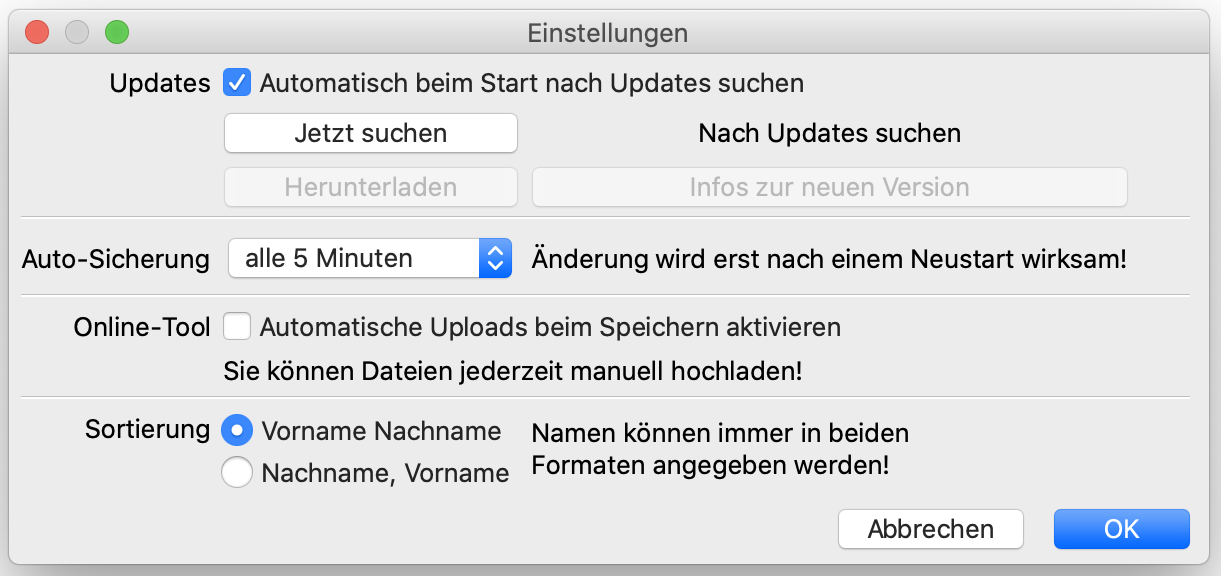
\includegraphics[width=\textwidth]{img/einstellungen}
	\caption{Das Fenster für die Programmeinstellungen.}
	\label{fig:einstellungen}
\end{figure}



\section{Updates}
Sie können eine automatische Suche nach neuen Versionen des Programms einstellen.
Ebenso können Sie sich die Informationen zur aktuellen Programmversion ansehen.

Die Funktion ist standardmäßig aktiviert.



\section{Auto-Sicherung}
Hier haben Sie die Möglichkeit einzustellen, ob das Program eine automatische Sicherung durchführen soll.
Bei dieser Funktion wird ihre originale Datei nicht überschrieben.
Stattdessen wird eine Datei mit dem gleichen Namen erstellt, der um \datei{.autosave.ako} ergänzt ist.
Diese Datei wird automatische beim manuellen Speichern entfernt.
Sollte das Programm unerwartet abstürzen, können Sie diese Datei direkt öffnen.

Standardmäßig ist diese Funktion deaktiviert!



\section{Online-Tool}
Hier können Sie einstellen, ob beim manuellen Speichern eine Listenansicht auf den Server hochgeladen wird.
Dies setzt voraus, dass die entsprechende Option in den Einstellungen für die \EPL-Datei auch aktiviert ist
(siehe \cref{einsatz:kalender:upload}).
Unabhängig von diesen Einstellungen können Sie die Ansicht jederzeit über die Exportfunktion (\cref{einsatz:kalender:export}) hochladen.

\begin{hinweis}
  Diese Funktion wird nur im Programm \Einsatz verwendet.
  Wenn die die Datei in \Personal speichern, wird keine Datei auf den Server geladen!
\end{hinweis}


\section{Anzeige Namen}
Es kann eingestellt werden, wie die Namen der Personen in der Mitgliederübersicht angezeigt und sortiert werden.
Die Änderung wird beim nächsten Aktualisieren der Mitgliederverwaltung wirksam und erfordert keinen Neustart.

\chapter{Sonstiges}\label{sonstiges}
\section{Informationen zum Update von Version 1.5 auf 1.6}
\label{sonstiges:1.5-1.6}
In Version 1.6 wurden verschiedene Neuerungen eingeführt, die eine gesonderte Betrachtung erfordern.
Diese Neuerungen werden im Folgenden beschrieben.


\paragraph{Personaldaten}
In der Personalverwaltung (siehe Kapitel~\ref{personal}) gibt es neben den verschiedenen persönlichen Daten auch ein Feld für die \emph{Betriebsdiensttauglichkeit}.
Dieses ist dafür vorgesehen sicherzustellen, dass nur Personal eingesetzt wird, dessen medizinische Tauglichkeit noch gültig ist.
Es ist nicht möglich Personal mit abgelaufener Tauglichkeit für eine betriebliche Aufgabe einzutragen.
Ist der Zeitpunkt für die Untersuchung unbekannt, wird das Personal aus medizinischer Sicht als tauglich angesehen.
Es liegt dann vollständig beim Bediener dies zu überwachen.

Ebenso kann für eine Person ein \emph{Austrittsdatum} angegeben werden.
Während dies im Allgemeinen nicht benötigt wird, kann diese Funktion dennoch bei (angehenden) ehemaligen Mitgliedern verwendet werden.
Somit kann die Person weiterhin im System registriert sein und muss nicht aus allen Aktivitäten entfernt werden.
Für diese Personen werden nach dem Austritt selbstverständlich keine Mindeststunden mehr berechnet.
Ebenso können sie nach dem Austritt auch nicht mehr für Arbeitseinsätze oder Fahrtage eingetragen werden.

Eine weitere Neuerung ist die \emph{Mitgliedsnummer}.
Beim erstmaligen Öffnen einer Datei, die mit einer früheren Programmversion erstellt wurde, wird jeder registrierten Person eine fortlaufende Nummer zugewiesen.
Diese Nummer kann nachträglich geändert werden, um sie an die eigene Bedürfnisse anzupassen.
Da naturgemäß jede Nummer nur einmal vergeben werden kann,
kann es beim Ändern der Nummer zu Kollisionen kommen.
Deshalb sollte bei der größten zuzuweisenden Nummer mit dem Ändern begonnen werden.
Dadurch wird die Nummer wieder für andere Personen freigegeben.
Wird eine Person neu angelegt,
so wird ihr automatisch die nächste Nummer größer als die aktuell größte vergebene Nummer zugewiesen.


\paragraph{Personaleintrag bei Aktivitäten}
Bei früheren Programmversionen war es nicht möglich eine Person mehrfach in einer Aktivität (Fahrtag oder Arbeitseinsatz) einzutragen.
Dies ist ab sofort möglich.
Allerdings muss hierzu die entsprechende Aufgabe der Person verschieden sein.
So kann zum Beispiel eine Person als Tf und als Zf eingetragen werden.
Allerdings sollte dann die Zeiten für die entsprechenden Tätigkeiten angepasst werden,
da sonst die Zeiten der Person mehrfach angerechnet werden (jeweils für jede Tätigkeit).




\section{Über das Dokument}
Die Bilder in dieser Dokumentation stammen von Bildern der Entwicklerversionen des Programms für Version 1.6.2 und aus früheren Versionen.
Dadurch können Programmobjekte und Funktionen leicht von denen in der veröffentlichten Version abweichen.

Eine aktuelle Version des Programms und weitere Informationen finden Sie der Webseite \url{http://epl.philipp-schepper.de}
oder im Repository unter \url{https://github.com/philjosch/Einsatzplaner}.


\part{Einsatzplaner}
\chapter{Übersichtskalender}
\section{Anlegen von Aktivitäten}
Um einen neuen Fahrtag anzulegen, klicken Sie auf den Knopf ``Neuer Fahrtag''.
Es wird ein Fahrtag mit dem aktuellen Datum angelegt.
Er wird in der Seitenleiste angezeigt.
Die Fahrtage werden, um einen schnelleren Überblick zubekommen in verschiedenen Farben anhand ihrer Art eingefärbt.

Ein neuer Arbeitseinsatz kann mit Hilfe des Knopfes ``Neuer Arbeitseinsatz'' angelegt werden, er wird ebenso wie die Fahrtage in der Liste und im Kalender angezeigt.

Ein Arbeitseinsatz kann auch direkt mit dem entsprechenden Datum durch einen Klick auf ``+'' im Kalender erstellt werden.


\section{Löschen von Aktivitäten}
Um eine Aktivität zu löschen, müssen Sie diese in der Seitenleiste auswählen und dann auf den Knopf ``Ausgewählten Eintrag löschen'' klicken.



\section{Navigation im Kalender}
Zurück: Blättert im Kalender einen Monat zurück\\
Vor:		Blättert im Kalender einen Monat vor \\
Heute:	Springt zum aktuellen Tag im Kalender \\
Eingabefeld:	Hier kann ein Datum direkt eingegeben werden


\section{Exportieren von Objekten}
Um Objekte zu exportieren, klicken Sie entweder auf den Knopf „Exportieren“ oder wählen im Menü ``Datei'' \nach ``Drucken\dots'' aus.
Alternativ ist diese Funktion auch mit dem Tastaturbefehl \texttt{cmd+P} beziehungsweise \texttt{ctrl+P} zu erreichen.
Weiteres hierzu finden Sie im Kapitel über die Export-Funktion.


\section{Das Datei-Menü}
Im folgenden werden die Einträge des ``Datei'' Menüs beschrieben.
\begin{description}
  \item[Neu]
  Erstellt ein neues Fenster mit einer leeren Einsatzplaner Instanz.

  \item[Öffnen \dots]
  Es wird ein Dialog geöffnet, mit dem eine \texttt{.ako}-Datei geöffnet werden kann.

  \item[Zuletzt Benutzt]
  Unter diesem Eintrag finden Sie die füf zuletzt verwendeten Dateien.
  Sie können direkt geöffnet werden.
  Ebenso können Sie bei Bedarf die Liste leeren.

  \item[Speichern]
  Die Datei wird an dem bisher bekannten Pfad gesichert, oder Sie werden nach einem Ort zum Sichern der Datei gefragt.

  \item[Sichern unter \dots]
  Sie können einen Ort auswählen, an dem die Datei gespeichert werden soll.

  Zum automatischen Sichern der Datei finden Sie weitere Informationen im Kapitel Einstellungen dieser Anleitung.

  \item[Stammdaten sichern unter \dots]
  Diese Funktion bietet die Möglichkeit, dass die unveränderlichen Daten exportiert werden; unter anderem Personaldaten und Einstellungen.
  Es werden keine Fahrtage oder Arbeitseinsätze gespeichert.
  Diese Funktion dupliziert sozusagen die aktuelle Datei und löscht dabei alle Fahrtage und Arbeitseinsätze.


  \item[Eigenschaften]
  Hier können Sie das Online-Tool aktivieren und konfigurieren.
  Weitere Informationen im entsprechenden Kapitel.

  \item[Schließen]
  Schließt das aktuelle Fenster.
  Wenn kein Fenster mehr geöffnet ist, wird das Programm beendet.

  \item[Exportieren \dots]
  Ruft die Exportfunktion auf.
  Weitere Funktionen in Kapitel \ref{export}.
\end{description}

\chapter{Fahrtage}\label{fahrtag}
\section{Allgemeines und Personal}
\begin{figure}[!h]
	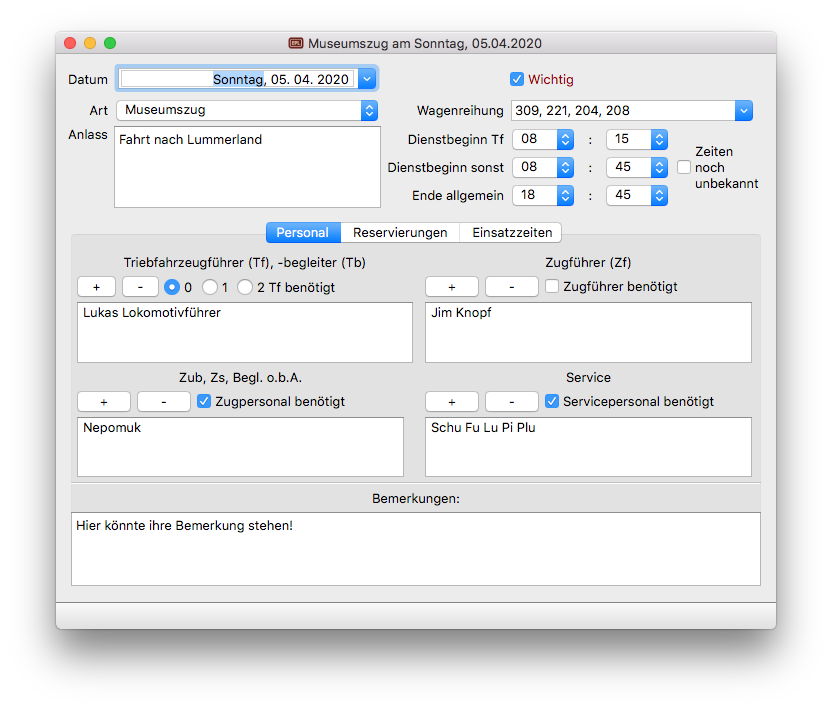
\includegraphics[width=\textwidth]{img/fahrtag_personal}
	\caption{Das Fenster eines Fahrtags mit geöffnetem Tab für das Personal.}
	\label{fig:fahrtag:personal}
\end{figure}
\paragraph{Allgemein}
Im oberen Bereich des Fensters können die grundlegenden Daten für einen Fahrtag eingegeben werden.
Eine Markierung als \emph{wichtig} wird beim Export des Fahrtages durch eine optische Hervorhebung gekennzeichnet.

Die Wagenreihung wirkt sich auf die Anzeige der Reservierungen aus und ist für die Personalplanung wichtig.
Es stehen bereits einige häufige Kombinationen der Wagen zur Verfügung.
Diese können aber auch beliebig verändert werden.
Dabei müssen die Wagen durch Kommata voneinander getrennt werden.

Sind die Zeiten für den Fahrtag noch unbekannt, können Sie das mit dem entsprechenden Häkchen kenntlich machen.
Ansonsten sind die Dienstzeiten anzugeben.

Der Anlass eines Fahrtages wird in der Kalenderansicht angezeigt.
Sodass bei einem Sonderzug schnell der Grund erkennbar ist.

\paragraph{Personal}
In den vier Listen können Tf, Zf, Zub und Begl.o.b.A.\ und Service-Personal eingetragen werden.
Für betriebliche Aufgaben (Tf, Tb, Zf) können nur Personen eingetragen werden, die die entsprechende Ausbildung haben.
(Siehe Kapitel~\ref{personal:einzelansicht})
Die Namen sind dabei wie folgt einzugeben: \texttt{Name; Bemerkung}.

Da Personal in Ausbildung die entsprechenden Berechtigungen noch nicht hat, können folgende Wörter in der Bemerkung verwendet werden, um diese Personen dennoch in der entsprechenden Liste einzutragen:
\begin{itemize}
	\item Azubi
	\item Ausbildung
	\item Tf-Ausbildung
	\item Zf-Ausbildung
	\item Tf-Unterricht
	\item Zf-Unterricht
	\item Weiterbildung
\end{itemize}
Ein Zugbegleiter ohne Ausbildung wird automatisch als Begl.o.b.A.\ geführt, sodass hier keine Unterscheidung vorgenommen werden muss.

Generell können nur Personen eingetragen werden, die im System bereits registriert wurden
(weiteres im Kapitel~\ref{personal}).
Auch hier gibt es wieder Ausnahmen, wenn einer der folgenden Begriffe in der Bemerkung erscheint:
\begin{itemize}
	\item Extern
	\item Führerstand
	\item FS
	\item Schnupperkurs
	\item ELF
	\item Ehrenlokführer
	\item ELF-Kurs
\end{itemize}
Darüber hinaus können weitere Bemerkungen eingegeben werden, die auch durch Strichpunkte voneinander getrennt sein dürfen.

\hinweis{Eine Person kann nicht mehrmals eingetragen werden!
Pro Aktivität kann jede Person nur eine Aufgabe übernehmen.
Sollte eine Person dennoch mehrere Funktionen wahrnehmen so kann dies nur in den Bemerkungen angegeben werden!}



\section{Reservierungen}
\begin{figure}[!h]
	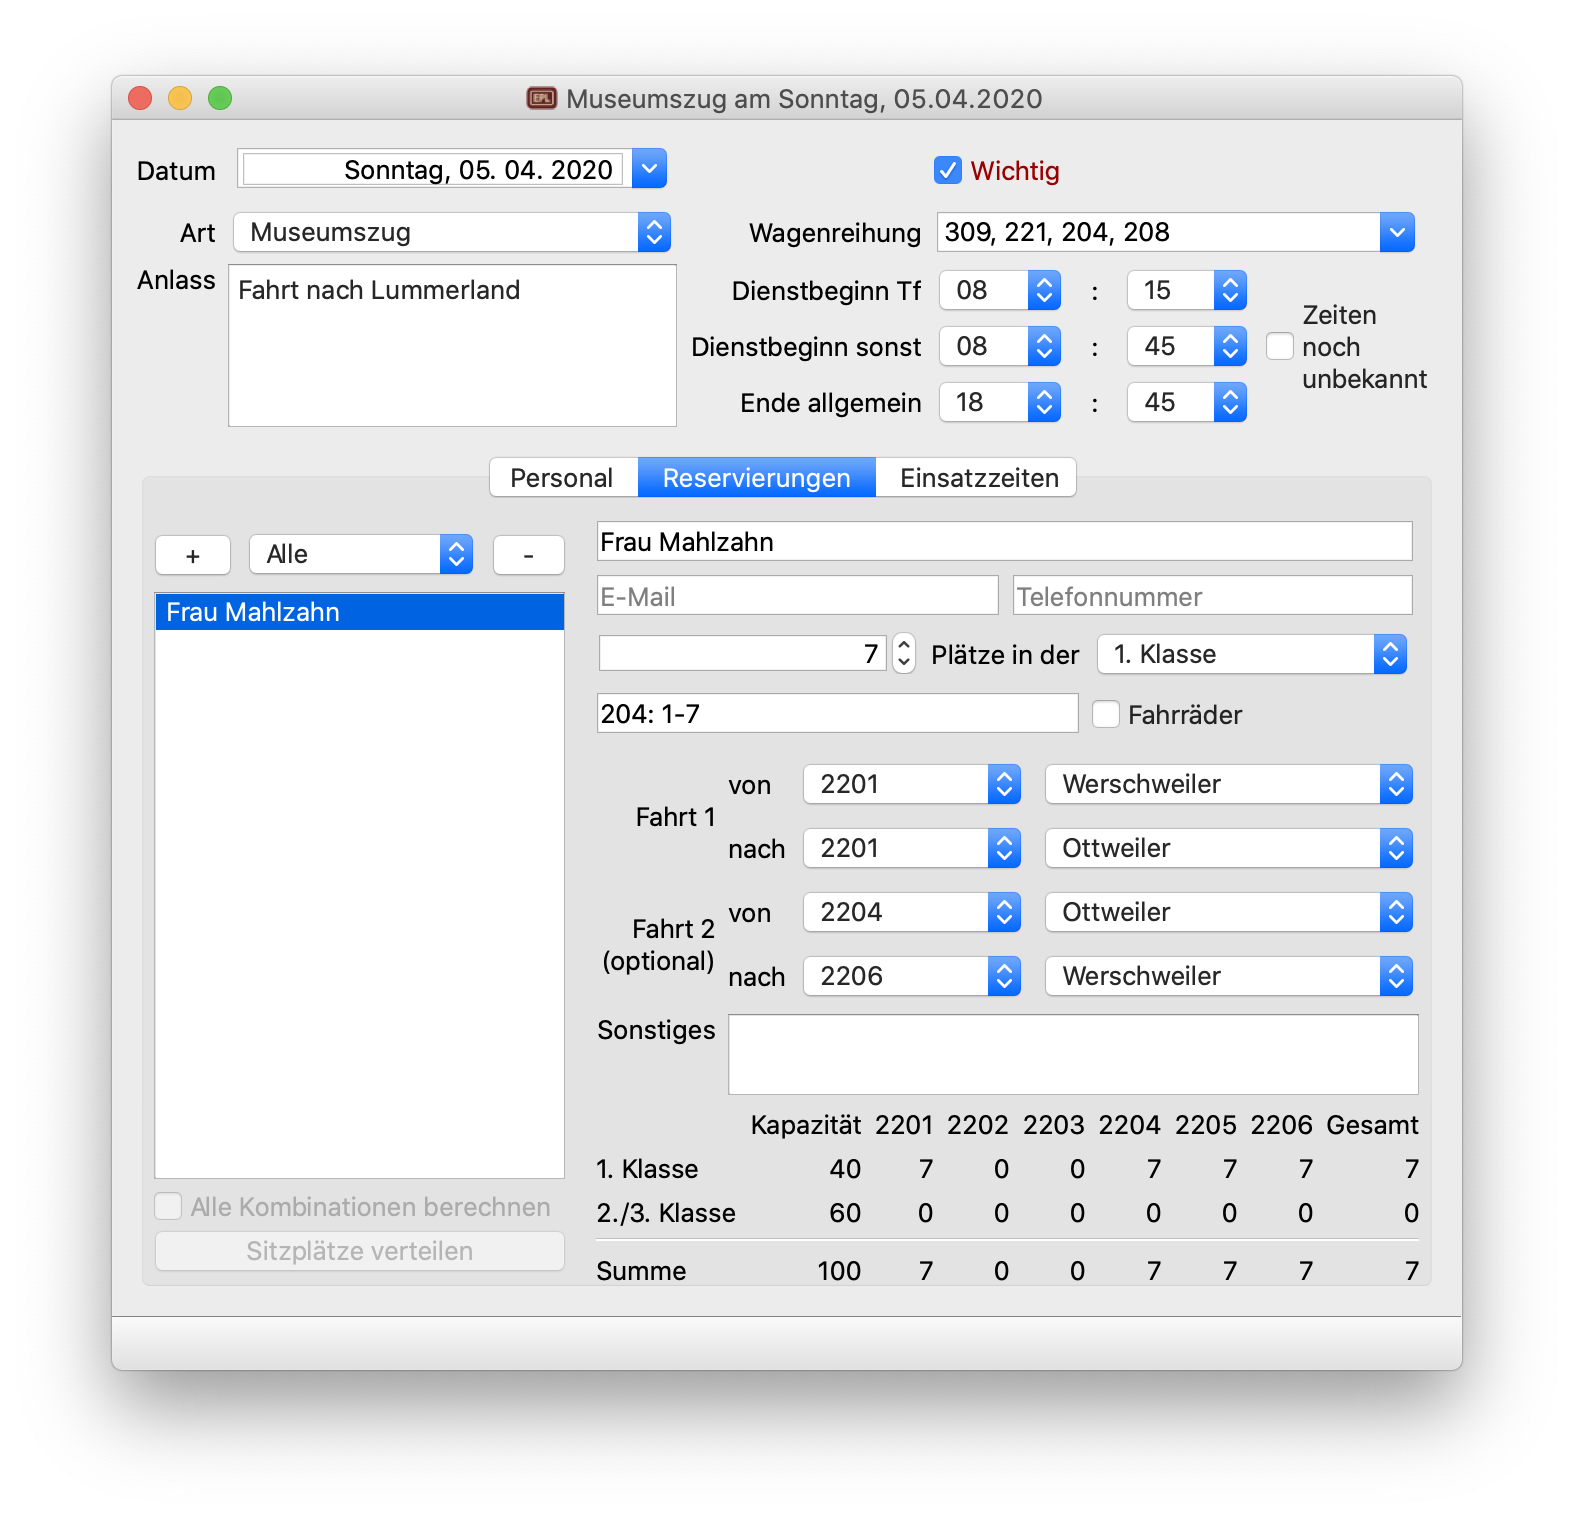
\includegraphics[width=\textwidth]{img/fahrtag_reservierungen}
	\caption{Das Fenster eines Fahrtags mit geöffnetem Tab für die Reservierungen.}
	\label{fig:fahrtag:reservierungen}
\end{figure}
Im unteren Teil besteht die Möglichkeit die Reservierungen zu verwalten.
Eine Reservierung können Sie bearbeiten, indem Sie doppelt auf den Eintrag in der Liste klicken.
Sie wird dann in das Formular geladen. Dort können Sie die zugehörigen Information ändern.


Die Sitzplätze müssen in folgendem Format angegeben werden:
Zuerst der Wagen und dann die Sitzplätze durch Kommata getrennt.
Aufeinanderfolgende Sitzplatznummern können Sie durch das Format Von-Bis schreiben (Beispiel: \texttt{208: 60-12}).
Wenn Sie Plätze in mehreren Wagen angeben möchten,
müssen Sie die Plätze durch einen Strickpunkt voneinander trennen
(Beispiel: \texttt{204: 1-40; 217: 1-30}).


Die Fahrtstrecke kann dabei in zwei nichtzusammenhängende Teilstrecken unterteilt werden.
Im Folgenden finden Sie mögliche Beispiele, wei Fahrtstrecken optimal eingegeben werden können:
\begin{itemize}
	\item Gruppe fährt in Zug 2202 von Ottweiler nach Schwarzerden und danach direkt wieder mit Zug 2203 zurück nach Ottweiler.\\
	Eingeben als:
	\begin{verbatim}Strecke 1  (2202 SOTW-SSWN) (Ottweiler)
           (2203 SSWN-SOTW) (Ottweiler)
Strecke 2  (-)              (-)
           (-)              (-)
	\end{verbatim}
	\item
	Eine andere Gruppe hat die gleiche Fahrstrecke, will aber eine Wanderung von Schwarzerden aus unternehmen und erst mit Zug 2205 wieder nach Ottweiler.
	Möglichkeit 1:
	\begin{verbatim}Strecke 1  (2202 SOTW-SSWN) (Ottweiler)
           (-)              (Schwarzerden)
Strecke 2  (2205 SSWN-SOTW) (Schwarzerden)
           (-)              (Ottweiler)
	\end{verbatim}
	Möglichkeit 2:
	\begin{verbatim}Strecke 1  (2203 SOTW-SSWN) (Ottweiler)
           (2203 SOTW-SSWN) (Schwarzerden)
Strecke 2  (2205 SSWN-SOTW) (Schwarzerden)
           (2205 SSWN-SOTW) (Ottweiler)
	\end{verbatim}
	\item
	Eine dritte Gruppe fährt von Schwarzerden nach Ottweiler in Zug 2201 und dann mit Zug 2202 von Ottweiler nach Fürth.
	Dort steigen Sie aus und fahren mit Zug 2204 wieder zurück nach Schwarzerden:
	\begin{verbatim}
Strecke 1  (2201 SSWN-SOTW) (Schwarzerden)
           (2202 SOTW-SSWN) (Fürth)
Strecke 2  (2204 SOTW-SSWN) (Fürth)
           (-)              (Schwarzerden)
	\end{verbatim}
\end{itemize}


\paragraph{Auswertung der Reservierungen}
Im linken unteren Teil des Fensters wird angezeigt, zu welchemn Grad die einzelnen Klassen des Zuges jeweils belegt sind.
Hier wird mit den Reservierungen gerechnet, denen ein fester Sitzplatz zugeordnet wurde.

Wenn Sie zu einer Reservierung noch keinen Sitzplatz angegeben haben, wird diese Reservierung nicht zur Berechnung der Belegung herangezogen.
Allerdings wird die Reservierung in die Gesamtzahl mit einbezogen.
Es kann also folgendes vorkommen:
\begin{verbatim}
	Belegung 1. Klasse  10/40 (25\%)
	Belegung 2. Klasse          --
	Belegung 3. Klasse  30/60 (50\%)
	Belegung Gesamt    60/100 (60\%)
\end{verbatim}


\paragraph{Automatische Sitzplatzverteilung}
Wenn Sie bei der Art des Fahrtags eine Nikolausfahrt ausgewählt haben, haben Sie die Möglichkeit die Sitzplätze automatisch durch einen Druck auf den Knopf "`Sitzplätze verteilen"' zu verteilen.
Der Vorgang dauert in der Regel wenige Sekunden.
Es kann aber auch unter Umständen mehrere Minuten dauern.
Warten Sie diese Zeit bitte ab!
Wir arbeiten ständig an einer Verbesserung des Algorithmus zur Verteilung der Sitzplätze.

\hinweis{Aktivieren Sie das Feld "`Alle Kombinationen berechnen"' nur, wenn Sie wenige Reservierungen angegeben haben (maximal 5-7),
denn durch diese Auswahl wird der Rechenaufwand erheblich vergrößert!}


\paragraph{Reservierungen exportieren}
Beim Export von "`normalen"' Fahrtagen werden die Reservierungen mit ausgegeben.
Da bei Nikolausfahrten sehr viele Reservierungen vorliegen, werden Sie nicht bei der Einzelansicht des Fahrtags angegeben.
Stattdessen können Sie, wie bei allen anderen Fahrtagen auch,
die Funktion "`Reservierungen drucken \dots"' und "`Reservierungen als PDF sichern \dots"' im Menü Fahrtag nutzen.
Bei dieser Funktion werden dann die Reservierungen nach Wagen geordnet ausgegeben.
Auch die Information über einen anderen als den Standard-Zustieg wird ausgegeben.

Eine grafische Ansicht der Sitzplatzverteilung ist aktuell noch nicht möglich.



\section{Weiteres Personal}
\begin{figure}[!h]
	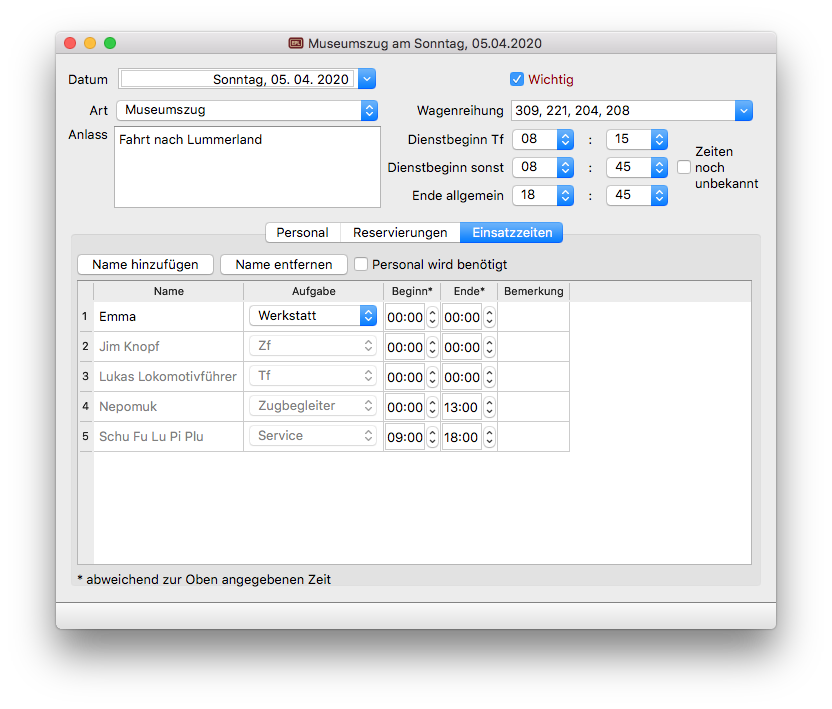
\includegraphics[width=\textwidth]{img/fahrtag_einsatzzeiten}
	\caption{Das Fenster eines Fahrtags mit geöffnetem Tab für das weitere Personal.}
	\label{fig:fahrtag:einsatzzeiten}
\end{figure}

In der Tabelle von Abbildung~\ref{fig:fahrtag:einsatzzeiten} erhalten Sie eine Übersicht über alle Personen,
die für diesen Fahrtag eingetragen wurden.
Zu jeder Person wird die Aufgabe angezeigt, die sie durchführt.
Die Arbeitszeit wird dann auf das entsprechende Konto angerechnet.
Es stehen die standardmäßigen Aufgaben (siehe Anhang~\ref{glossar}) zum Einstellen zur Verfügung.

Personen die betriebliche oder regelmäßige Aufgaben haben und somit bereits im Reiter Personal in eine Liste eingetragen wurden, werden hier auch angezeigt.
Allerdings können nur die Einsatzzeiten dieser Personen verändert werden.
Diese Personen müssen in den entsprechenden Listen gelöscht werden.


Die Spalten "`Beginn"' und "`Ende"' dienen dazu, Uhrzeiten anzugeben, wenn Personen nicht für den kompletten angegebenen Zeitraum geholfen haben.
So kann man eine frühere Endzeit eingeben, wenn zum Beispiel eine Person nur am Vormittag half.
Die Zeit der Lokführer wird automatisch anhand von "`Dienstbeginn Tf"' berechnet,
sodass hier kein manueller Eintrag vorgenommen werden muss.



\section{Menü}
Im Menü Fahrtag gibt es die Möglichkeit die Einzelansicht des geöffneten Fahrtages zu exportieren.
Ebenso können die Reservierungen ausgegeben werden oder der Fahrtag nach einer Sicherheitsanfrage komplett gelöscht werden.

\chapter{Arbeitseinsätze}\label{arbeitseinsatz}
\begin{figure}[h!]
	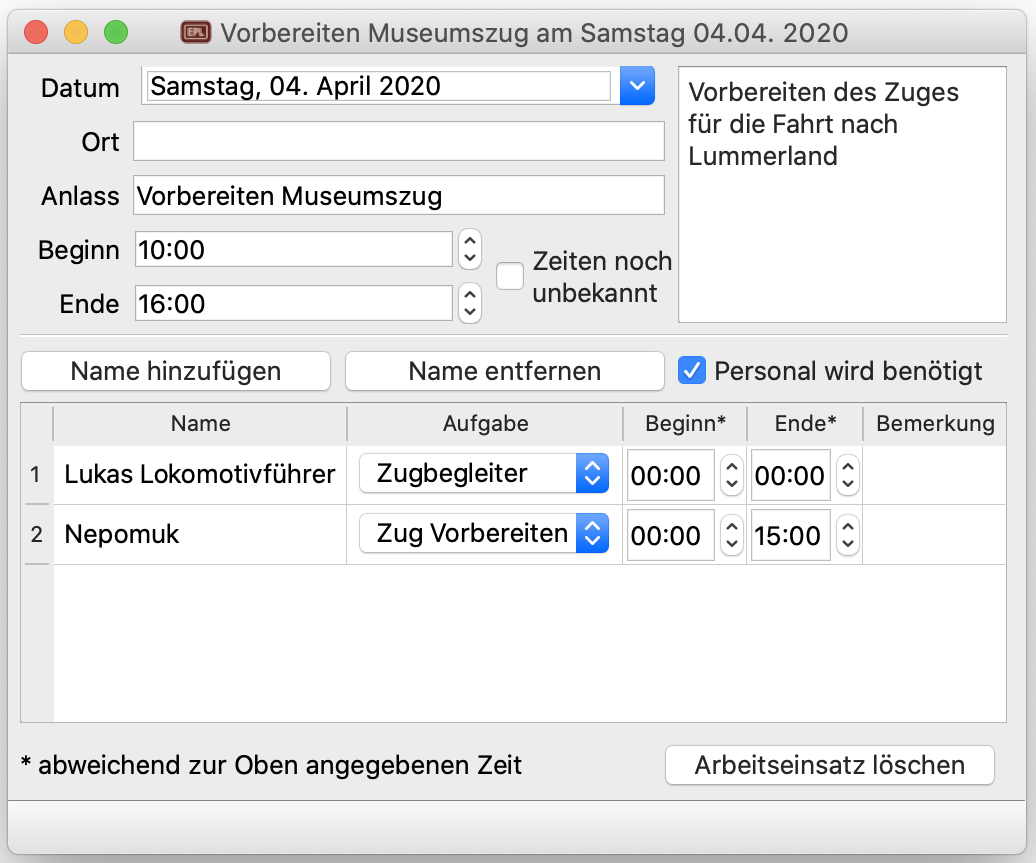
\includegraphics[width=\textwidth]{img/arbeitseinsatz}
	\caption{Das Fenster eines Arbeitseinsatzes.}
	\label{fig:arbeitseinsatz}
\end{figure}
Die Eingabe der Daten erfolgt hier analog zur Eingabe der Daten in das Fenster für einen Fahrtag.
Allerdings sind hier alle Personen in die Liste einzutragen.
Das Programm versucht anhand des Anlasses die Aufgabe bereits möglichst genau zu bestimmen.

\chapter{\neu{Mitglieder}}\label{personal}
Im Kopf des Fensters kann eingestellt werden welche Personen angezeigt werden sollen.
Ebenso kann durch einen Knopfdruck eine E-Mail an alle angezeigten Personen erstellt werden.
Werden bei dieser Aktion Personen gefunden, für die keine Mailadresse angegeben ist,
so können die angegebenen Postadressen in einer CSV-Datei gespeichert werden.
Diese Daten können dann z.B.\ für Serienbriefe genutzt werden.

\section{\neu{Einsatzzeiten}}\label{personal:zeiten}
\begin{figure}[!h]
	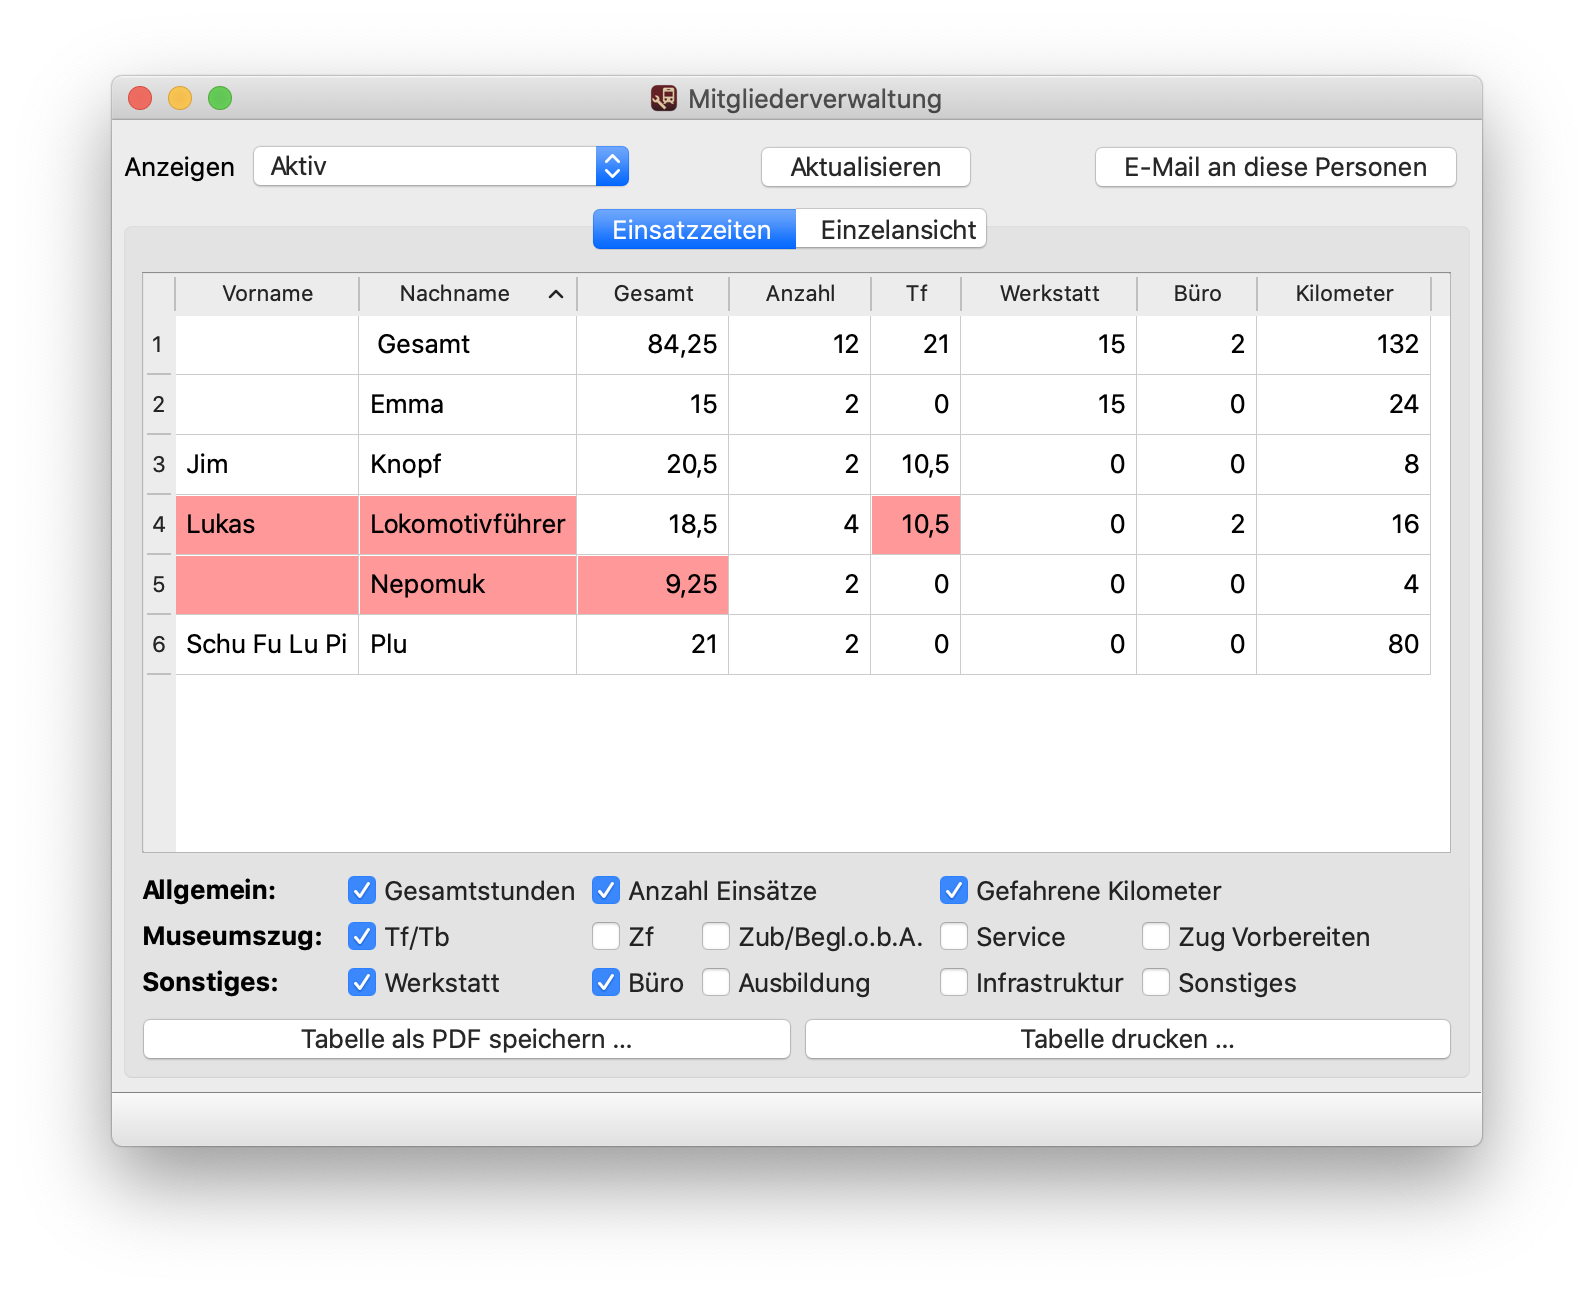
\includegraphics[width=\textwidth]{img/personal_gesamt}
	\caption{\neu{Die Mitgliederverwaltung mit den Einsatzzeiten.}}
	\label{fig:personal:zeiten}
\end{figure}
In der Tabelle von Abbildung~\ref{fig:personal:zeiten} wird eine Übersicht über alle in der Kopfzeile ausgewählten Personen gegeben.
Die Einfärbung erfolgt anhand der mindestens zu erbringenden Stunden.
Rot bedeutet hierbei, dass die Person ihre Stunden noch nicht erbracht hat.
Eine weiße Markierung bestätigt, dass die Mindeststunden erbracht wurden, oder keine solchen gefordert sind (z.B.\ bei passiven Mitglieder).
\neu{Für aktive Mitglieder gilt, dass sie in die Kategorie "`Aktiv mit Stunden"' fallen, sobald die Mindeststunden für "`Gesamt"' erreicht wurden.
Die persönlichen Mindeststunden für Lokführer werden hierbei nicht berücksichtigt.
Dennoch werden diese Personen auch rot markiert.}
Passive Mitglieder, die Stunden geleistet haben, werden grün markiert.
Durch einen Doppelklick auf den Eintrag einer Person in der Tabelle wird die entsprechende Einzelansicht geöffnet.


Mit Hilfe der Auswahlkästchen können die verschiedenen Spalten mit den Zeiten der Personen ein- und ausgeblendet werden, die dann auch entsprechend sortiert werden können.
Ebenso wird die Summe der jeweiligen Spalten in der Zeile "`Gesamt"' angegeben.
Diese Zeile ist in der Ausgabe ebenso enthalten.


Mit den Knöpfen "`Tabelle als PDF speichern \dots"' und "`Tabelle drucken \dots"' kann man die Daten der Tabelle exportieren.
Diese Funktionen sind auch im Menü "`Exportieren"' verfügbar.


\paragraph{Mindeststunden}
Die Mindeststunden können über den Eintrag "`Mindeststunden \dots"' im Menü "`Personalmanagement"' bearbeitet werden.
Der sich öffnende Dialog ist in Abbildung~\ref{fig:personal:mindeststunden} dargestellt.

\begin{figure}[!h]
	\centering
	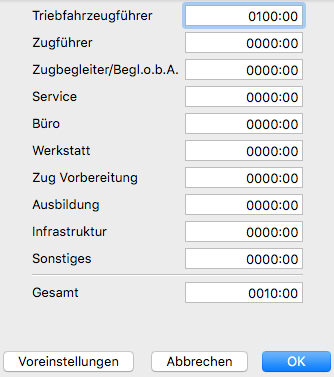
\includegraphics[width=0.5\textwidth]{img/personal_mindeststunden}
	\caption{Der Dialog zum Ändern der Mindesstunden.}
	\label{fig:personal:mindeststunden}
\end{figure}

Standardmäßig sind 10 Stunden für alle aktiven Mitglieder eingestellt.
Personal mit Ausbildung zum Lokführer muss 100 Stunden als Lokführer ableisten.
Die Werte für jedes Konto können beliebig geändert werden.

Die Mindeststunden für Ausbildung werden nur für Personal mit einer betrieblichen Ausbildung und bestehender Tauglichkeit angewendet.




\section{Einzelansicht}\label{personal:einzelansicht}
\begin{figure}[!h]
	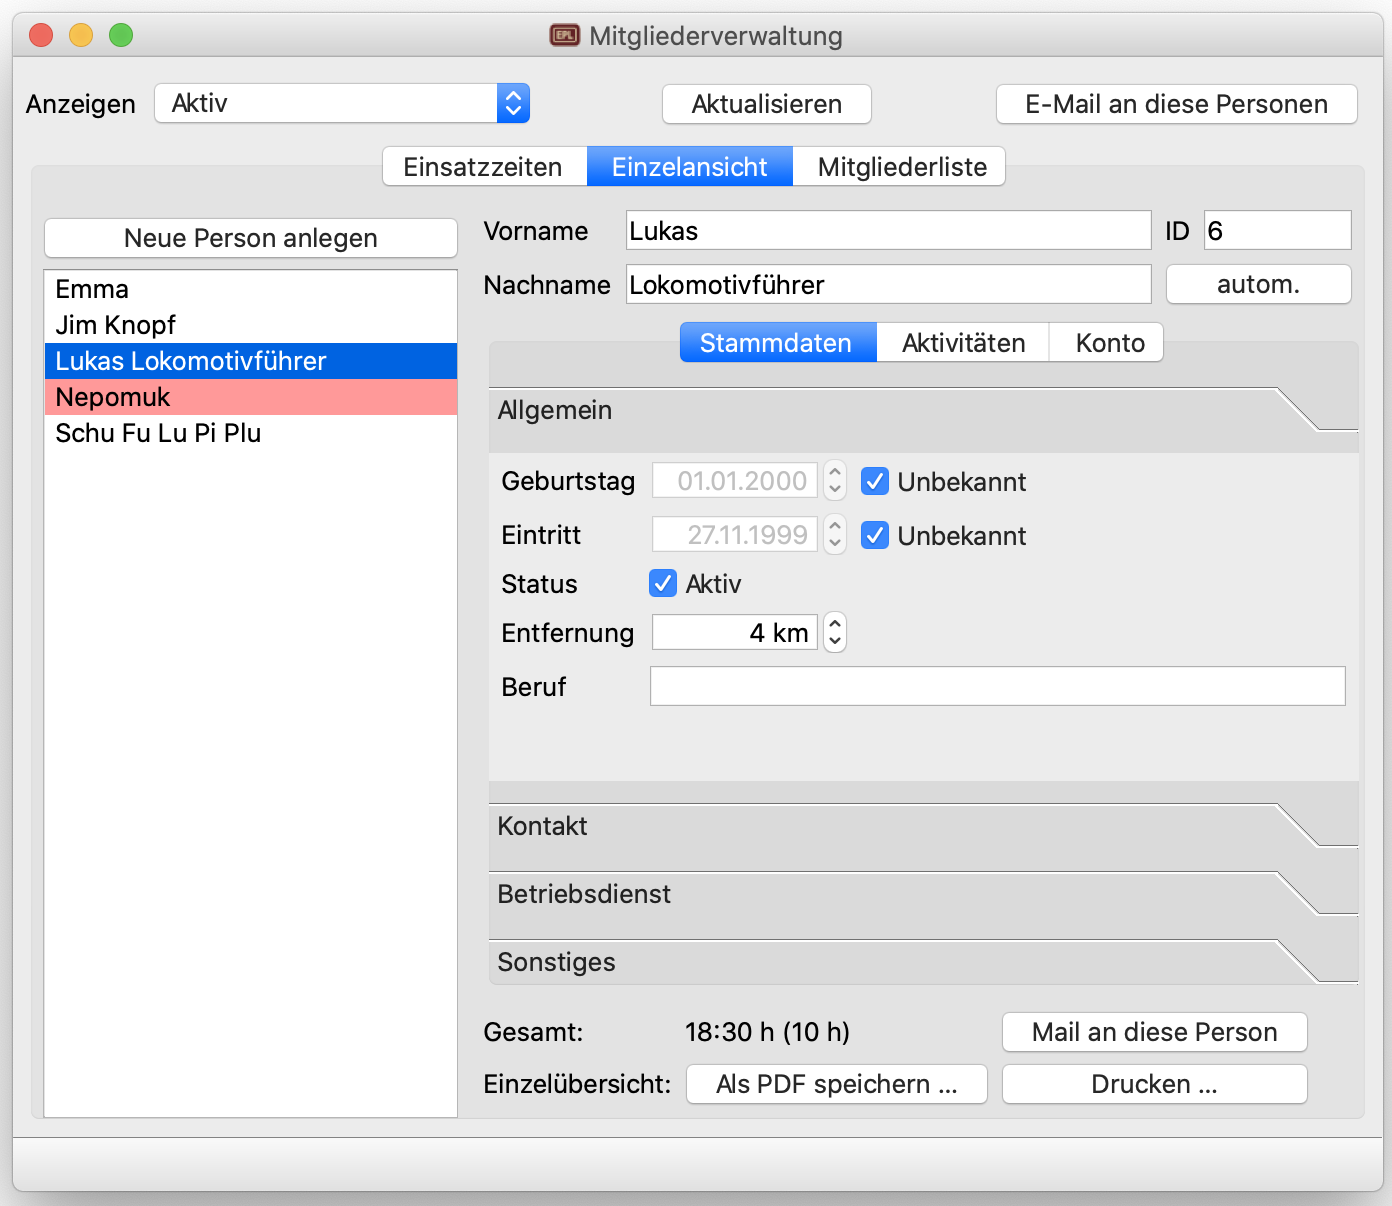
\includegraphics[width=\textwidth]{img/einzelansicht_stammdate_allgemein}
	\caption{Die Einzelansicht mit geöffnetem Reiter für die Stammdaten}
	\label{fig:personal:einzel:stammdaten}
\end{figure}
Das Fenster mit geöffneter Einzelansicht ist in Abbildung~\ref{fig:personal:einzel:stammdaten} zu sehen.
In der Liste sind alle Personen gelistet, die nach der Kopfzeile des Fenster angezeigt werden sollen.
Die farbliche hervorhebung erfolgt analog zur Gesamtübersicht.
Im oberen Teil können der Name und die Mitgliedsnummer der Person verändert werden.
Alternativ zu manuellen Eingabe der Nummer, kann auch eine solche automatisch zugewiesen werden.
Dabei wird die nächst größere Zahl der aktuell höchsten Mitgliedsnummer verwendet.
Naturgemäß kann eine Nummer nicht doppelt vergeben werden.

Mit den Knöpfen "`Als PDF speichern \dots"' und "`Drucken\dots"' kann eine Übersicht der aktuellen Person ausgegeben werden.
Dort werden dann die Aktivitäten einzeln mit den jeweiligen Zeiten aufgelistet.
Diese Ansicht enthält nur wenige persönliche Informationen.


\paragraph{Stammdaten}
Unter \emph{Allgemein} können das Geburtsdatum, Eintrittsdatum und der Status (Aktiv/Passiv) der Person angegeben werden.
Das Feld "`Entfernung"' wird verwendet die gefahrene Wegstrecke aufgrund der Aktivitäten zu berechnen.
Ebenso kann der erlernte Beruf der Person eingegeben werden.

Unter \emph{Kontakt} besteht die Möglichkeit eine Postadresse, Telefonnummmer und Mailadresse einzutragen.
Ebenso besthet die Möglichkeit anzugebene, ob das Mitglied seine Einwilligung zur Veröffentlichung für Vereinsmitglieder und Betriebsangehörige erteilt hat.

Der Bereich \emph{Betriebsdienst} bietet die Möglichkeit betriebliche Ausbildungen zu erfassen.
Das Feld Tauglichkeit dient dazu anzugeben, bis wann die aktuelle Tauglichkeitsuntersuchung gilt (letzter Tag der Gültigkeit).
Personal, dessen Tauglichkeit nicht mehr gegeben ist, wird wie Personal ohne betriebliche Ausbildung behandelt.

Unter \emph{Sonstiges} gibt es ein Feld für Bemerkungen und die Möglichkeit den Austritt einer Person einzutragen.
Auch kann dort die Person aus dem System entfernt werden.

\hinweis{Eine Person kann erst dann gelöscht werden, wenn Sie in keinen Aktivitäten mehr eingetragen ist.
Siehe nächster Absatz.}


\begin{figure}[!h]
	\centering
	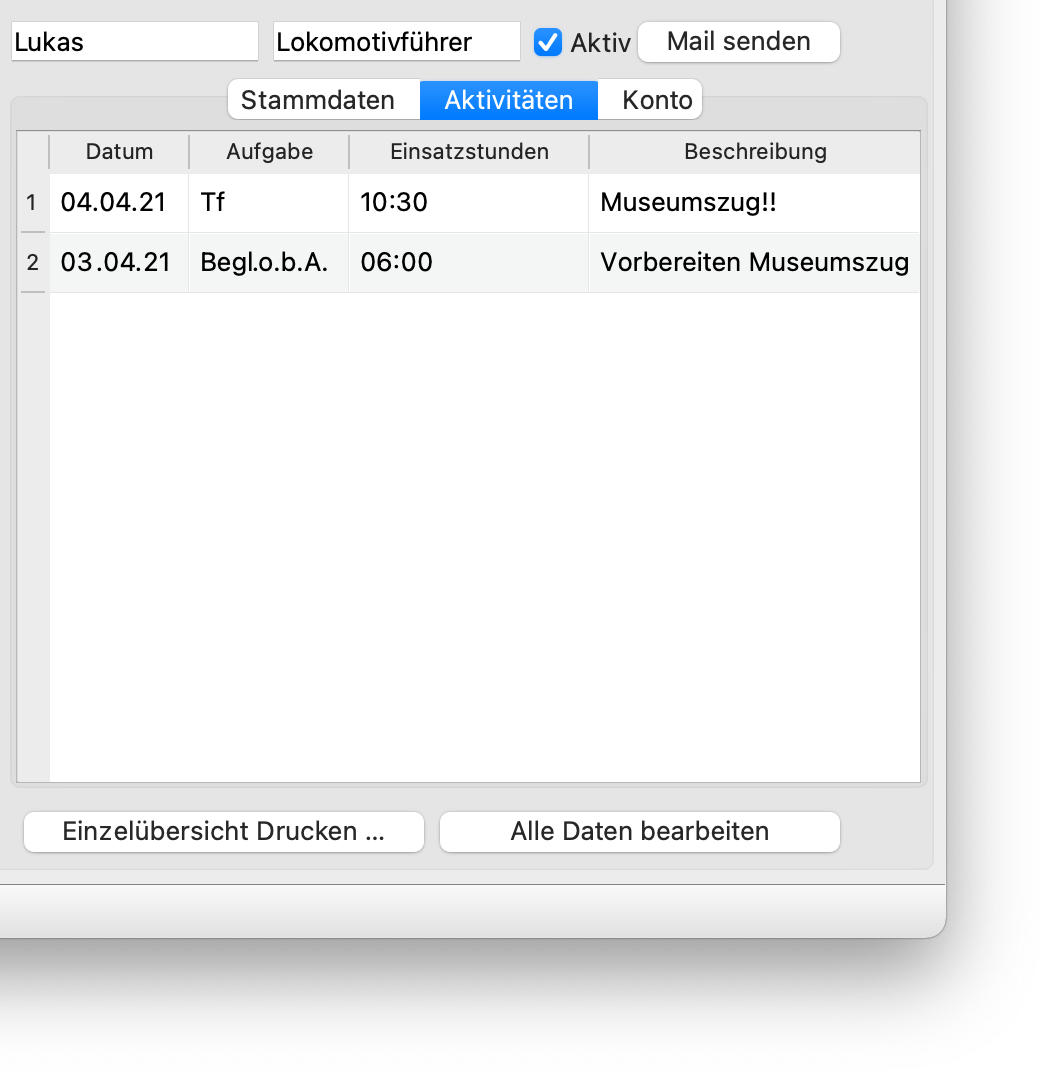
\includegraphics[width=.75\textwidth]{img/einzelansicht_aktivitaeten}
	\caption{Die Einzelansicht mit geöffnetem Reiter für die Aktivitäten}
	\label{fig:personal:einzel:aktivitaeten}
\end{figure}
\paragraph{Aktivitäten}
Der Reiter,
des in Abbildung~\ref{fig:personal:einzel:aktivitaeten} dargestellten Fensters,
zeigt eine Tabelle mit den Aktivitäten,
an denen die ausgewählte Person mitgeholfen hat.


\begin{figure}[!h]
	\centering
	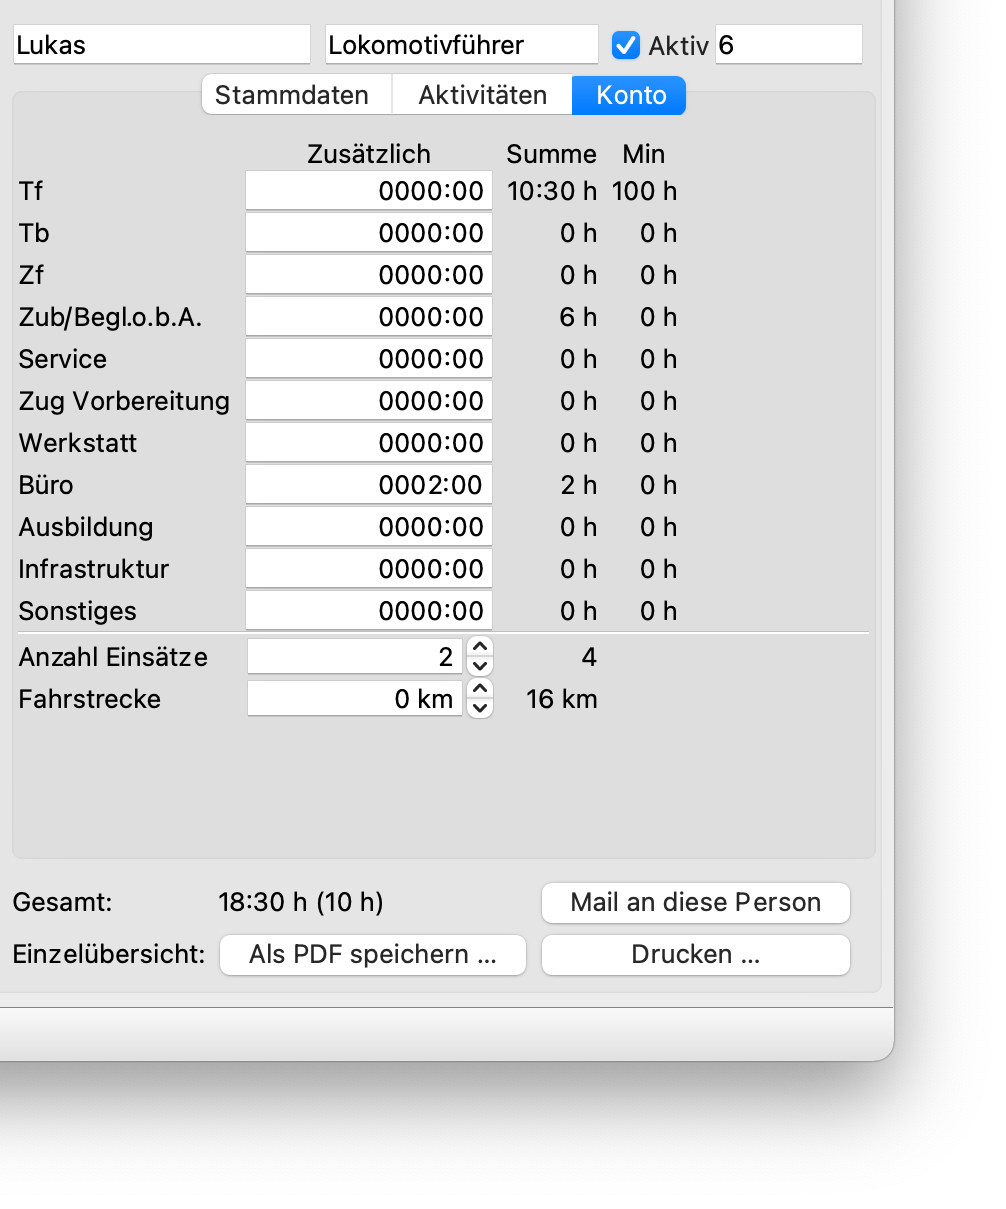
\includegraphics[width=.75\textwidth]{img/einzelansicht_konto}
	\caption{Die Einzelansicht mit geöffnetem Reiter für das Zeitenkonto}
	\label{fig:personal:einzel:konto}
\end{figure}
\paragraph{Konto}
Die Übersicht in Abbildung~\ref{fig:personal:einzel:konto} enthält die Zeiten aufgeteilt nach den verschiedenen Zeit-Konten.
Ebenso können hier zusätzliche Stunden und Kilometer eintragen werden,
welche die Person geleistet hat, aber keiner im System erfassten Aktivität zuzuordnen sind.
Die Anzahl der zusätzlichen Aktivitäten kann ebenfalls erfasst werden.
Ebenso kann man sehen, in welchen Gebieten die Person ihre Pflichtstunden erfüllt hat und wieviele Mindeststunden Sie jeweils in den Gebieten erbringen muss.


\hinweis{Für alle Darstellungen und Berechnungen werden nur die Zeiten angerechnet, die bisher auch wirklich abgeleistet wurden,
also deren Datum in der Vergangenheit lag.}


\section{\neu{Mitgliederliste}}\label{personal:mitglieder}
\begin{figure}[!h]
	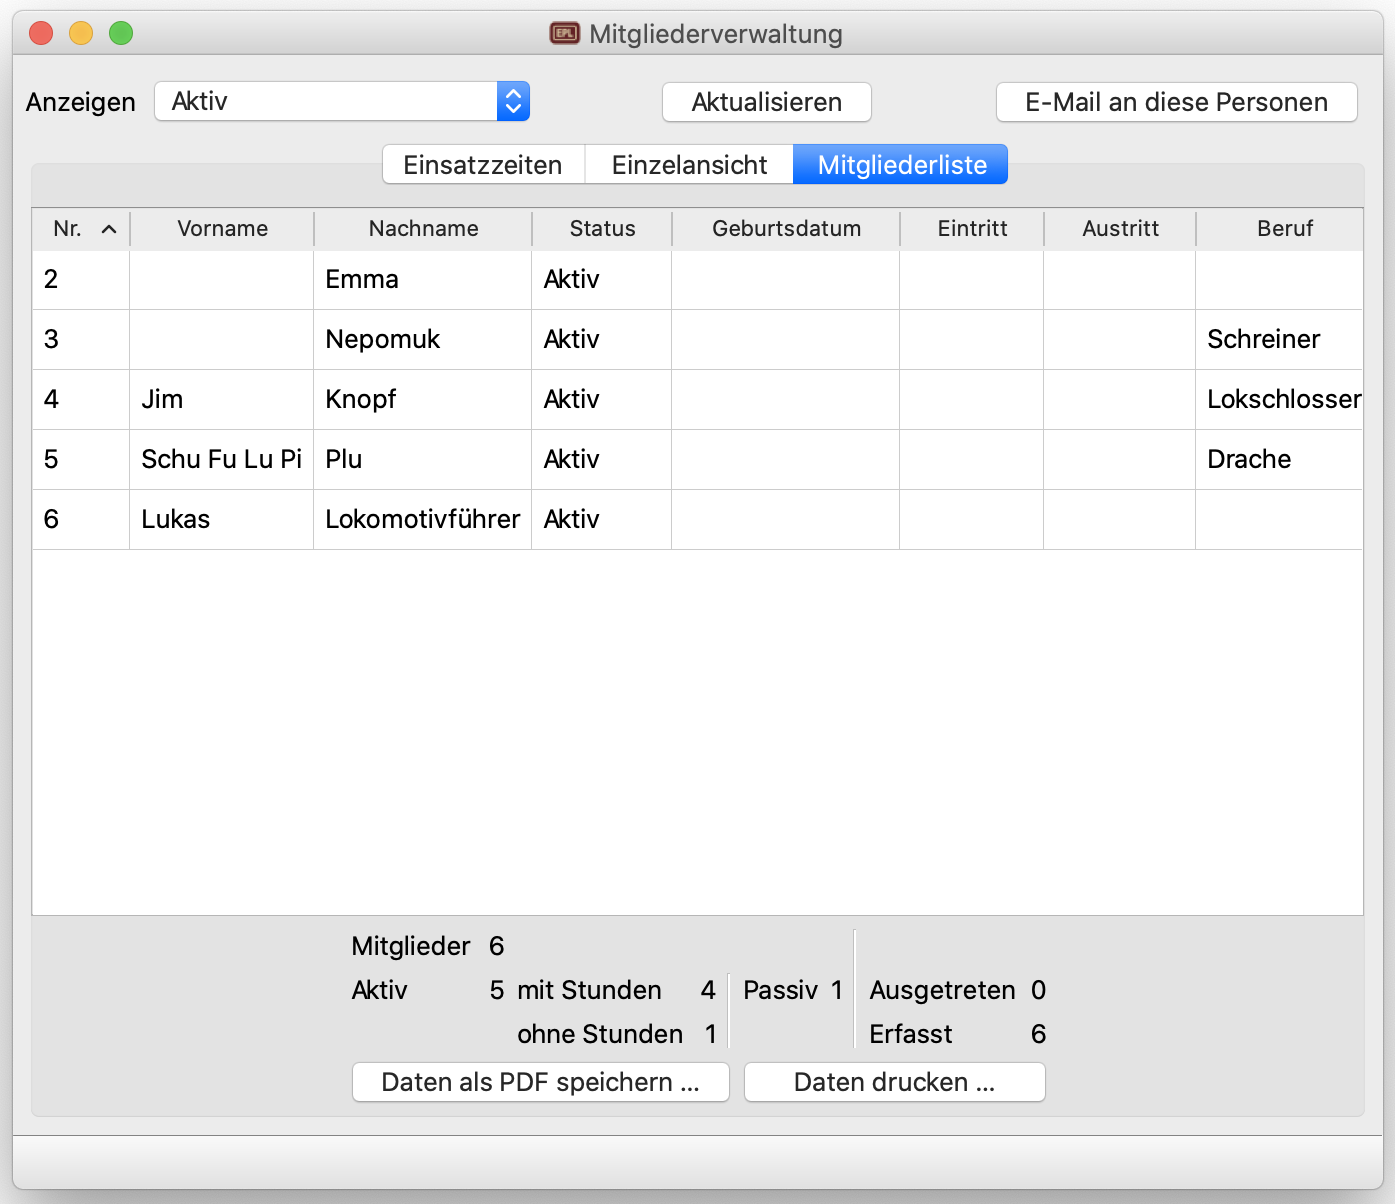
\includegraphics[width=\textwidth]{img/mitgliederliste}
	\caption{\neu{Die Mitgliederliste mit allen ausgewählten Mitgliedern.}}
	\label{fig:personal:mitglieder}
\end{figure}
\neu{In der Tabelle aus Abbildung~\ref{fig:personal:mitglieder} werden alle gespeicherten Daten der ausgewählten Mitglieder angezeigt.
Diese Tabelle kann über das Menü "`Exportieren"' unter dem Punkt "`Mitgliederliste"' ausgegeben werden.
Die Ausgabe ist auch als CSV-Datei möglich, sodass die Daten in anderen Programmen verarbeitet werden können.

Ebenso besteht die Möglichkeit über den Eintrag "`Personalblatt"' die Daten eines Mitglieds bzw.\ aller angezeigten Personen auszugeben.
Hierbei wird für jede Person eine Seite erzeugt und kann somit auch für jede Person getrennt gespeichert werden.

Darüber hinaus wird im unteren Bereich des Fensters eine Statistik der aktuellen und ausgetretenen Mitglieder angezeigt.
}


\part{Personalplaner}

\chapter{\neu{Mitglieder}}\label{personal}
Im Kopf des Fensters kann eingestellt werden welche Personen angezeigt werden sollen.
Ebenso kann durch einen Knopfdruck eine E-Mail an alle angezeigten Personen erstellt werden.
Werden bei dieser Aktion Personen gefunden, für die keine Mailadresse angegeben ist,
so können die angegebenen Postadressen in einer CSV-Datei gespeichert werden.
Diese Daten können dann z.B.\ für Serienbriefe genutzt werden.

\section{\neu{Einsatzzeiten}}\label{personal:zeiten}
\begin{figure}[!h]
	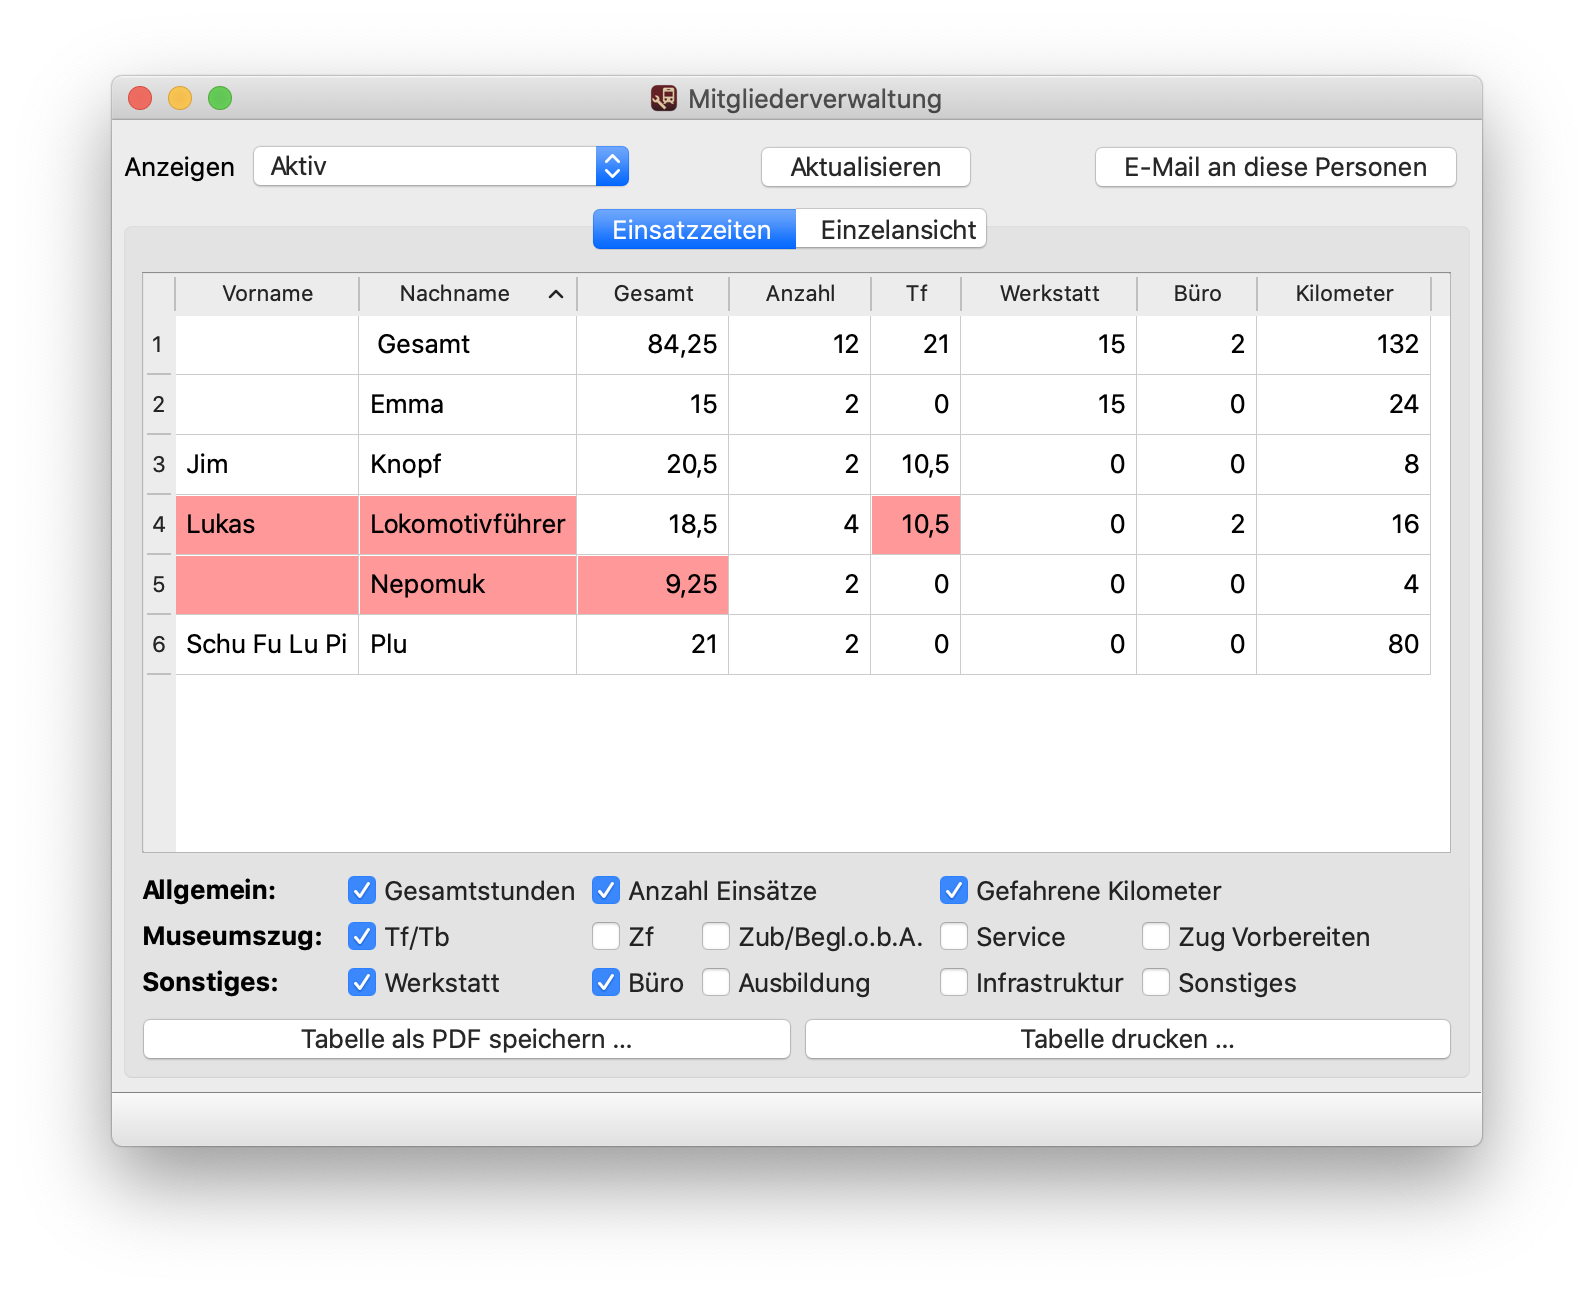
\includegraphics[width=\textwidth]{img/personal_gesamt}
	\caption{\neu{Die Mitgliederverwaltung mit den Einsatzzeiten.}}
	\label{fig:personal:zeiten}
\end{figure}
In der Tabelle von Abbildung~\ref{fig:personal:zeiten} wird eine Übersicht über alle in der Kopfzeile ausgewählten Personen gegeben.
Die Einfärbung erfolgt anhand der mindestens zu erbringenden Stunden.
Rot bedeutet hierbei, dass die Person ihre Stunden noch nicht erbracht hat.
Eine weiße Markierung bestätigt, dass die Mindeststunden erbracht wurden, oder keine solchen gefordert sind (z.B.\ bei passiven Mitglieder).
\neu{Für aktive Mitglieder gilt, dass sie in die Kategorie "`Aktiv mit Stunden"' fallen, sobald die Mindeststunden für "`Gesamt"' erreicht wurden.
Die persönlichen Mindeststunden für Lokführer werden hierbei nicht berücksichtigt.
Dennoch werden diese Personen auch rot markiert.}
Passive Mitglieder, die Stunden geleistet haben, werden grün markiert.
Durch einen Doppelklick auf den Eintrag einer Person in der Tabelle wird die entsprechende Einzelansicht geöffnet.


Mit Hilfe der Auswahlkästchen können die verschiedenen Spalten mit den Zeiten der Personen ein- und ausgeblendet werden, die dann auch entsprechend sortiert werden können.
Ebenso wird die Summe der jeweiligen Spalten in der Zeile "`Gesamt"' angegeben.
Diese Zeile ist in der Ausgabe ebenso enthalten.


Mit den Knöpfen "`Tabelle als PDF speichern \dots"' und "`Tabelle drucken \dots"' kann man die Daten der Tabelle exportieren.
Diese Funktionen sind auch im Menü "`Exportieren"' verfügbar.


\paragraph{Mindeststunden}
Die Mindeststunden können über den Eintrag "`Mindeststunden \dots"' im Menü "`Personalmanagement"' bearbeitet werden.
Der sich öffnende Dialog ist in Abbildung~\ref{fig:personal:mindeststunden} dargestellt.

\begin{figure}[!h]
	\centering
	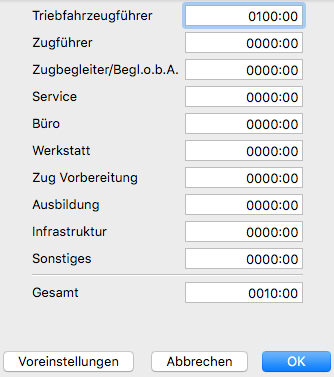
\includegraphics[width=0.5\textwidth]{img/personal_mindeststunden}
	\caption{Der Dialog zum Ändern der Mindesstunden.}
	\label{fig:personal:mindeststunden}
\end{figure}

Standardmäßig sind 10 Stunden für alle aktiven Mitglieder eingestellt.
Personal mit Ausbildung zum Lokführer muss 100 Stunden als Lokführer ableisten.
Die Werte für jedes Konto können beliebig geändert werden.

Die Mindeststunden für Ausbildung werden nur für Personal mit einer betrieblichen Ausbildung und bestehender Tauglichkeit angewendet.




\section{Einzelansicht}\label{personal:einzelansicht}
\begin{figure}[!h]
	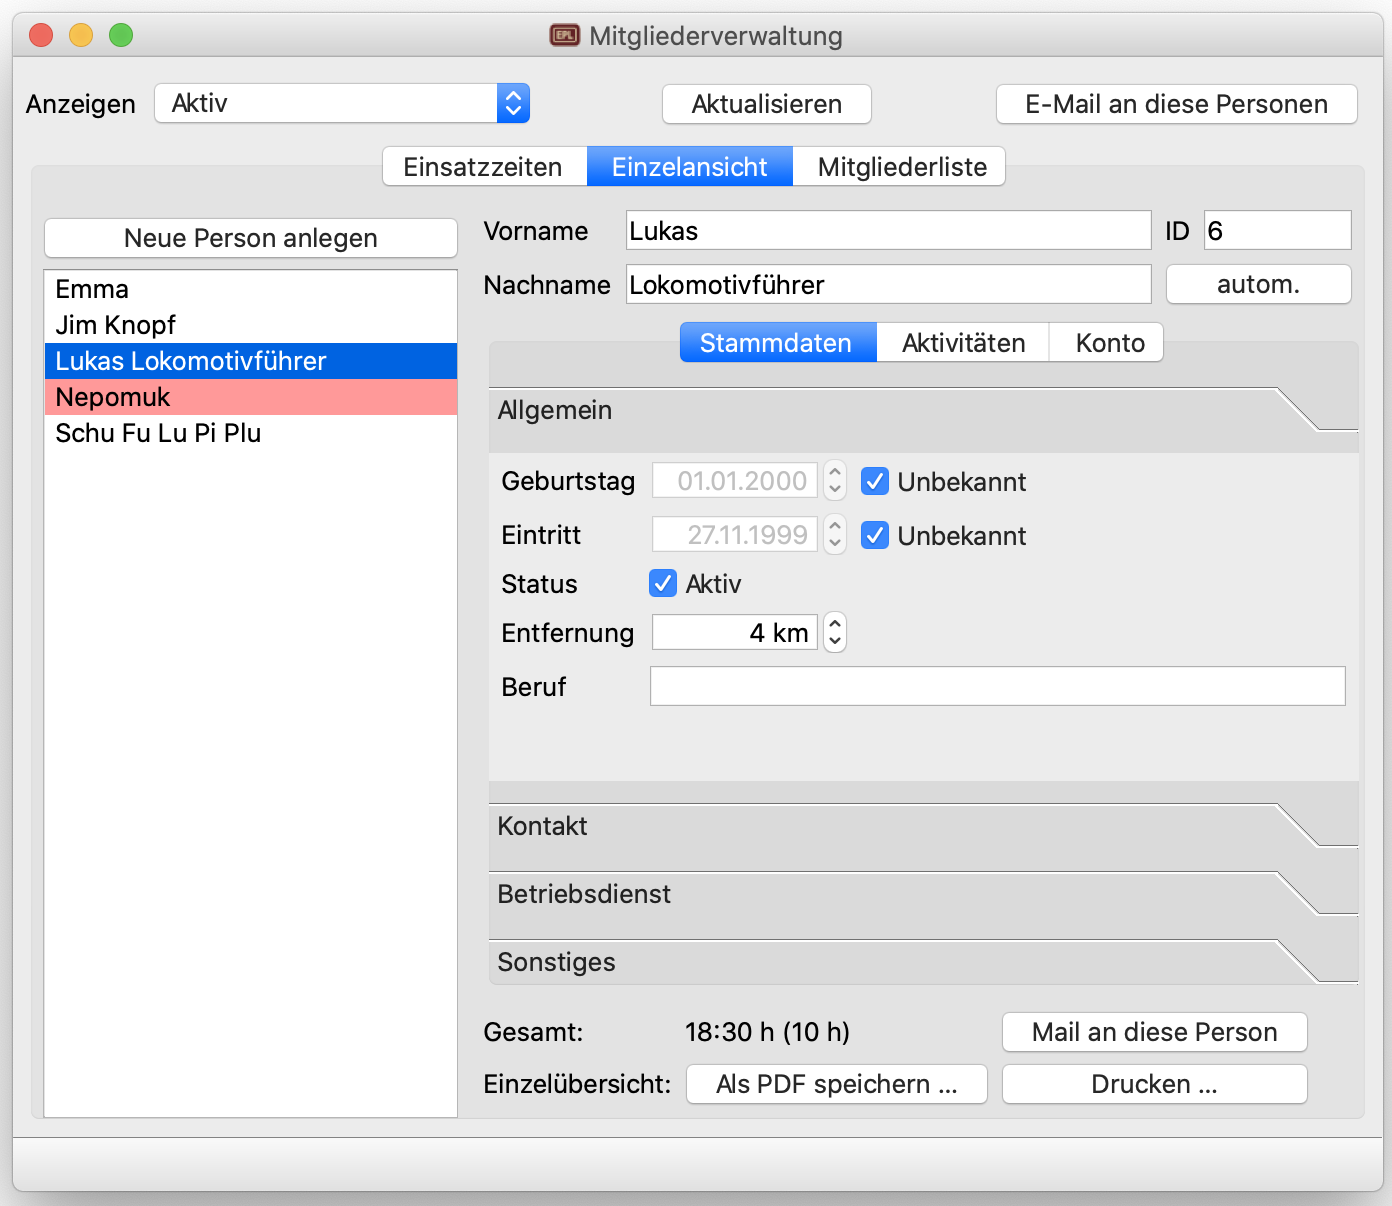
\includegraphics[width=\textwidth]{img/einzelansicht_stammdate_allgemein}
	\caption{Die Einzelansicht mit geöffnetem Reiter für die Stammdaten}
	\label{fig:personal:einzel:stammdaten}
\end{figure}
Das Fenster mit geöffneter Einzelansicht ist in Abbildung~\ref{fig:personal:einzel:stammdaten} zu sehen.
In der Liste sind alle Personen gelistet, die nach der Kopfzeile des Fenster angezeigt werden sollen.
Die farbliche hervorhebung erfolgt analog zur Gesamtübersicht.
Im oberen Teil können der Name und die Mitgliedsnummer der Person verändert werden.
Alternativ zu manuellen Eingabe der Nummer, kann auch eine solche automatisch zugewiesen werden.
Dabei wird die nächst größere Zahl der aktuell höchsten Mitgliedsnummer verwendet.
Naturgemäß kann eine Nummer nicht doppelt vergeben werden.

Mit den Knöpfen "`Als PDF speichern \dots"' und "`Drucken\dots"' kann eine Übersicht der aktuellen Person ausgegeben werden.
Dort werden dann die Aktivitäten einzeln mit den jeweiligen Zeiten aufgelistet.
Diese Ansicht enthält nur wenige persönliche Informationen.


\paragraph{Stammdaten}
Unter \emph{Allgemein} können das Geburtsdatum, Eintrittsdatum und der Status (Aktiv/Passiv) der Person angegeben werden.
Das Feld "`Entfernung"' wird verwendet die gefahrene Wegstrecke aufgrund der Aktivitäten zu berechnen.
Ebenso kann der erlernte Beruf der Person eingegeben werden.

Unter \emph{Kontakt} besteht die Möglichkeit eine Postadresse, Telefonnummmer und Mailadresse einzutragen.
Ebenso besthet die Möglichkeit anzugebene, ob das Mitglied seine Einwilligung zur Veröffentlichung für Vereinsmitglieder und Betriebsangehörige erteilt hat.

Der Bereich \emph{Betriebsdienst} bietet die Möglichkeit betriebliche Ausbildungen zu erfassen.
Das Feld Tauglichkeit dient dazu anzugeben, bis wann die aktuelle Tauglichkeitsuntersuchung gilt (letzter Tag der Gültigkeit).
Personal, dessen Tauglichkeit nicht mehr gegeben ist, wird wie Personal ohne betriebliche Ausbildung behandelt.

Unter \emph{Sonstiges} gibt es ein Feld für Bemerkungen und die Möglichkeit den Austritt einer Person einzutragen.
Auch kann dort die Person aus dem System entfernt werden.

\hinweis{Eine Person kann erst dann gelöscht werden, wenn Sie in keinen Aktivitäten mehr eingetragen ist.
Siehe nächster Absatz.}


\begin{figure}[!h]
	\centering
	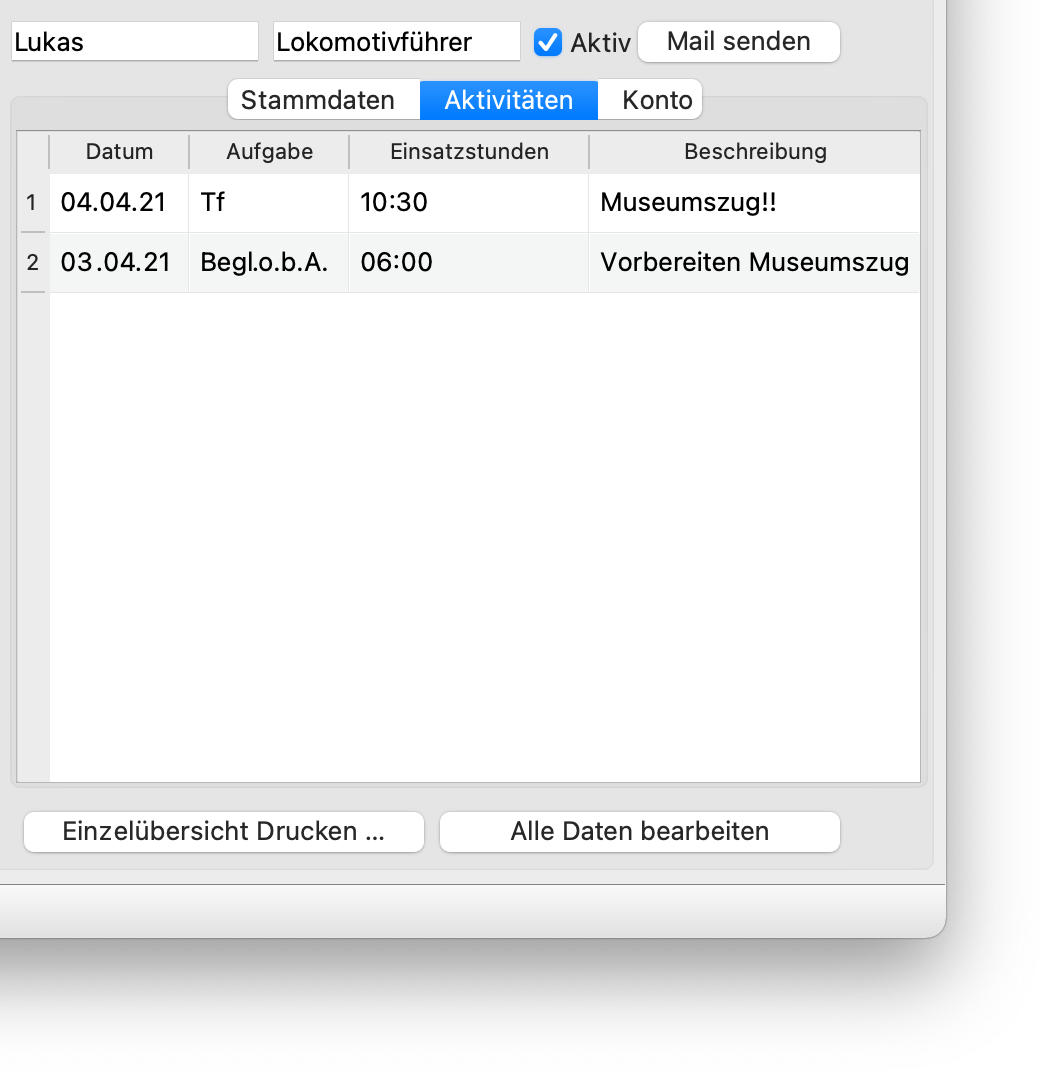
\includegraphics[width=.75\textwidth]{img/einzelansicht_aktivitaeten}
	\caption{Die Einzelansicht mit geöffnetem Reiter für die Aktivitäten}
	\label{fig:personal:einzel:aktivitaeten}
\end{figure}
\paragraph{Aktivitäten}
Der Reiter,
des in Abbildung~\ref{fig:personal:einzel:aktivitaeten} dargestellten Fensters,
zeigt eine Tabelle mit den Aktivitäten,
an denen die ausgewählte Person mitgeholfen hat.


\begin{figure}[!h]
	\centering
	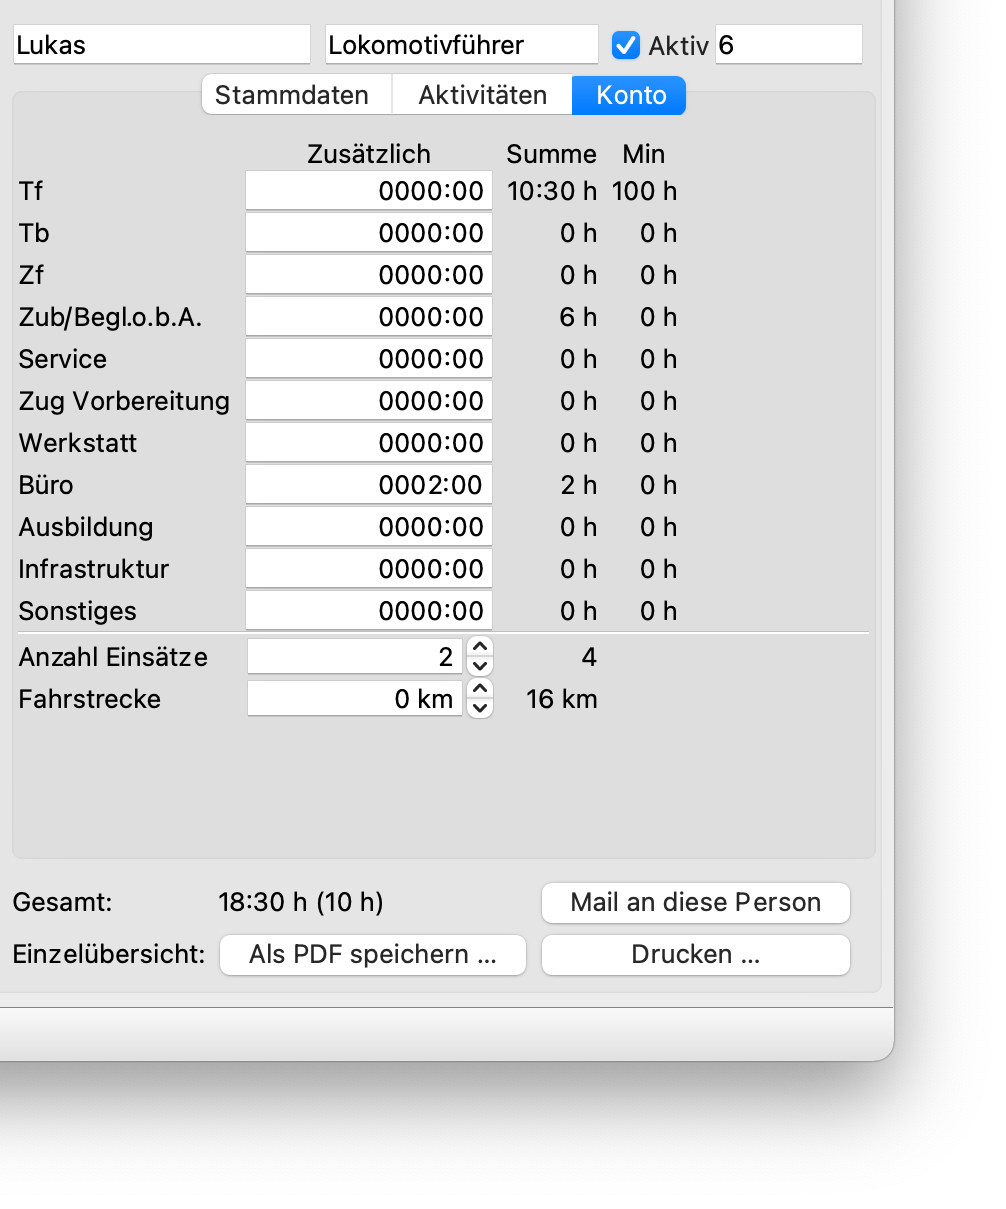
\includegraphics[width=.75\textwidth]{img/einzelansicht_konto}
	\caption{Die Einzelansicht mit geöffnetem Reiter für das Zeitenkonto}
	\label{fig:personal:einzel:konto}
\end{figure}
\paragraph{Konto}
Die Übersicht in Abbildung~\ref{fig:personal:einzel:konto} enthält die Zeiten aufgeteilt nach den verschiedenen Zeit-Konten.
Ebenso können hier zusätzliche Stunden und Kilometer eintragen werden,
welche die Person geleistet hat, aber keiner im System erfassten Aktivität zuzuordnen sind.
Die Anzahl der zusätzlichen Aktivitäten kann ebenfalls erfasst werden.
Ebenso kann man sehen, in welchen Gebieten die Person ihre Pflichtstunden erfüllt hat und wieviele Mindeststunden Sie jeweils in den Gebieten erbringen muss.


\hinweis{Für alle Darstellungen und Berechnungen werden nur die Zeiten angerechnet, die bisher auch wirklich abgeleistet wurden,
also deren Datum in der Vergangenheit lag.}


\section{\neu{Mitgliederliste}}\label{personal:mitglieder}
\begin{figure}[!h]
	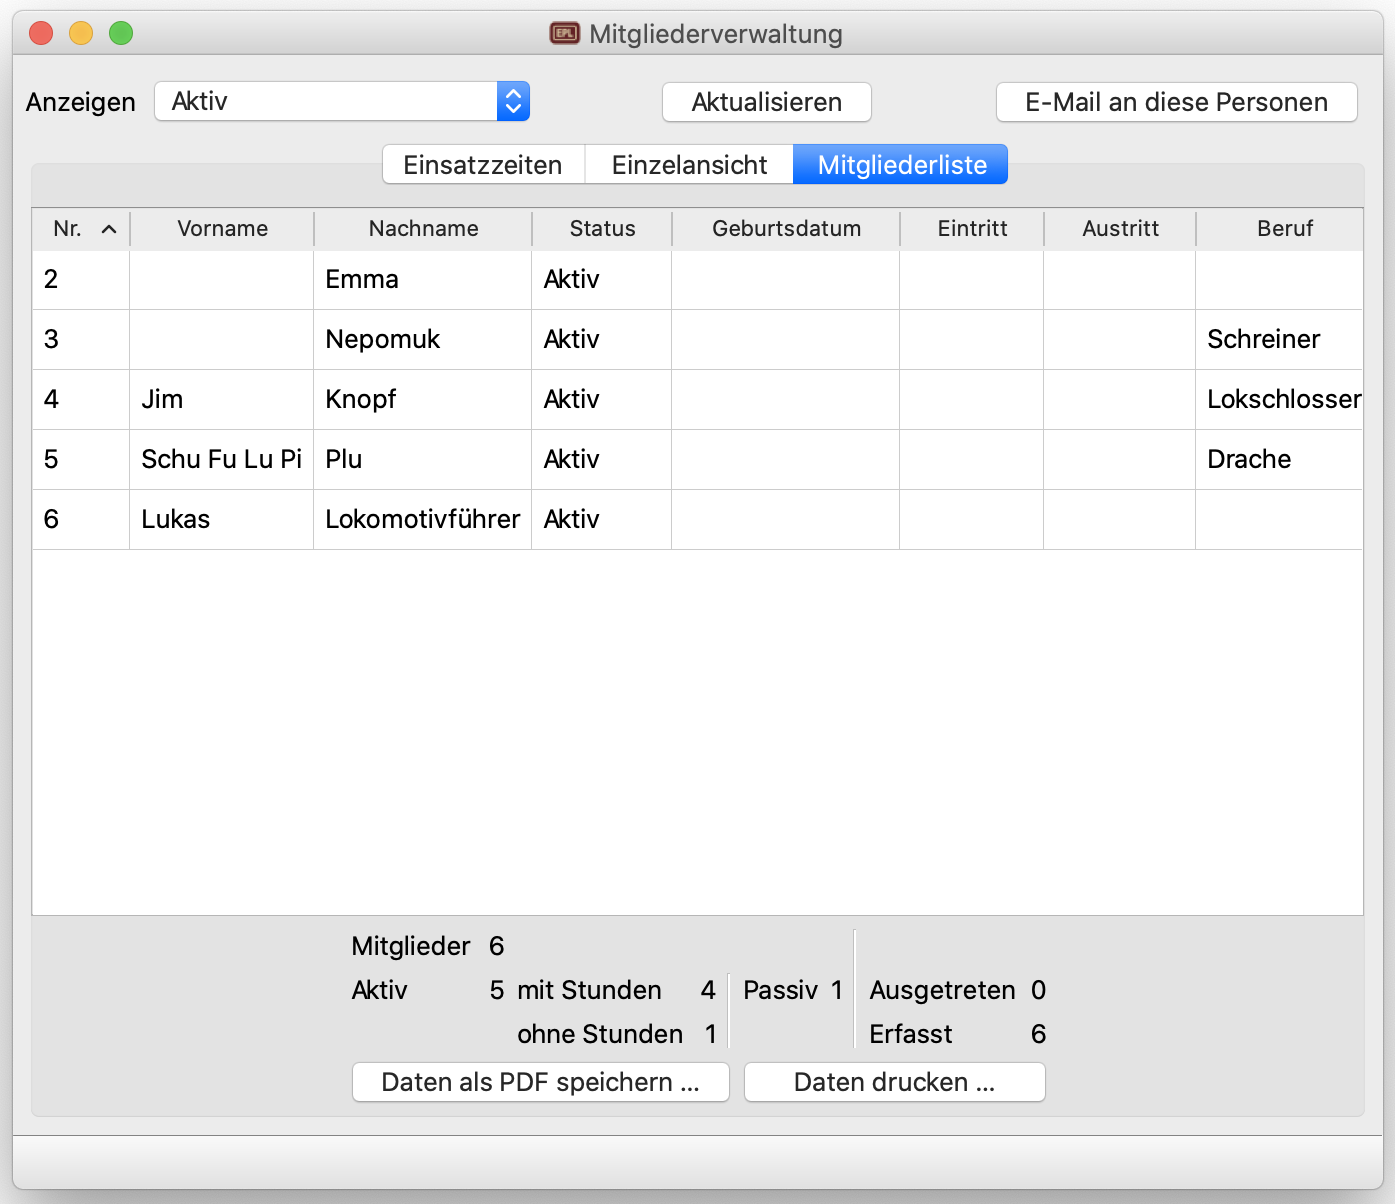
\includegraphics[width=\textwidth]{img/mitgliederliste}
	\caption{\neu{Die Mitgliederliste mit allen ausgewählten Mitgliedern.}}
	\label{fig:personal:mitglieder}
\end{figure}
\neu{In der Tabelle aus Abbildung~\ref{fig:personal:mitglieder} werden alle gespeicherten Daten der ausgewählten Mitglieder angezeigt.
Diese Tabelle kann über das Menü "`Exportieren"' unter dem Punkt "`Mitgliederliste"' ausgegeben werden.
Die Ausgabe ist auch als CSV-Datei möglich, sodass die Daten in anderen Programmen verarbeitet werden können.

Ebenso besteht die Möglichkeit über den Eintrag "`Personalblatt"' die Daten eines Mitglieds bzw.\ aller angezeigten Personen auszugeben.
Hierbei wird für jede Person eine Seite erzeugt und kann somit auch für jede Person getrennt gespeichert werden.

Darüber hinaus wird im unteren Bereich des Fensters eine Statistik der aktuellen und ausgetretenen Mitglieder angezeigt.
}

\chapter{Einzelansicht Mitglied}\label{personal:person}
Das Fenster in \cref{fig:personal:person} zeigt das Standardfenster für die Bearbeitung der Personendaten.
Im Kopf werden der Name und die Mitgliedsnummer angezeigt und können geändert werden.
Beim Erstellen einer Person wird automatisch, die nächsthöhere Mitgliedsnummer vergeben, als aktuell vorhanden.
Ein Ändern der Mitgliedsnummer ist nur möglich, wenn die Nummer nicht bereits vergeben ist.

Für juristische Personen, die als Fördermitglieder aufgenommen sind, kann der Vorname freigelassen werden.
Es genügt hierbei den Nachnamen anzugeben.

\begin{figure}[!h]
  \centering
	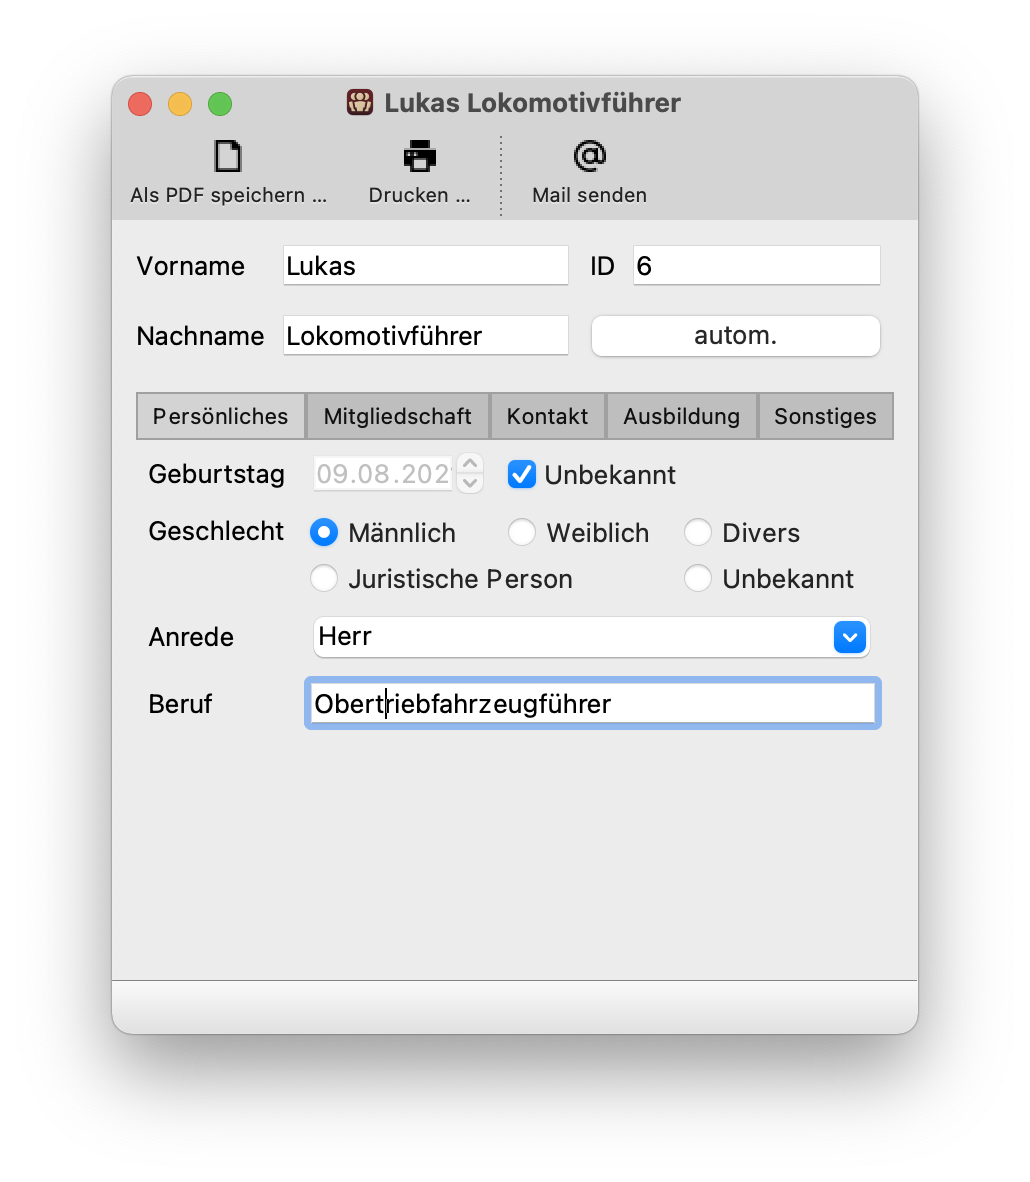
\includegraphics[width=0.75\textwidth]{img/personal-person}
	\caption{Das Fenster zum Bearbeiten der Daten eines Mitglieds.}
	\label{fig:personal:person}
\end{figure}


Im unteren Bereich des Fensters stehen verschiedene Reiter zur Verfügung,
über welche die persönlichen Daten abgerufen und verändert werden können.


\paragraph{Person Löschen}
Sie können über das Menü \aktion{Person} die Person aus dem System entfernen.
Dies ist nur möglich, wenn sie bei keiner Aktivität mehr eingetragen ist.
Ist eine Person aus dem Verein ausgetreten, ist es \textbf{nicht} erforderlich sie zu löschen.
Stattdessen kann die Person als ausgetreten markiert und das Austrittsdatum vermerkt werden.
Somit bleibt die Person weiterhin im System erhalten und wird auch bei den jeweiligen Aktivitäten noch mit ausgegeben.


\paragraph{Betriebsdienst}
Für den Betriebsdienst kann eine Datum eingegeben werden, dass beschreibt bis wann die betriebliche Tauglichkeitsuntersuchung gültig ist.
Liegt für den Tag einer Aktivität keine Tauglichkeit vor, kann die Person nicht in der entsprechenden Kategorie eingetragen werden (z.B.\ als Tf oder Zf).
Für Zugbegleiter wird dann automatisch eine Eintragung als Begl.o.b.A.\ eingetragen.


\paragraph{Export}
Über das Menü \aktion{Export} kann das Stammdatenblatt der geöffneten Person exportiert werden.
Das Dokument enthält alle personenbezogenen Daten aus der EPL-Datei.
Es enthält jedoch keine Informationen zu Aktivitäten und geleisteten Stunden.


\part{EPL-Server}\label{server}
\chapter{Upload-Tool}\label{server:upload}
Zur Installation des Tools auf einem Server benötigen Sie eine nicht veraltete Version von PHP.
Die benötigten Dateien können von der Webseite des Programs (siehe \cref{epl:alg:sonstiges}) heruntergeladen werden.

Das Tool besteht aus der Konfigurationsdatei \datei{config.php} und dem eigentlichen Programm \datei{load.php}.
Der Name der Datei \datei{load.php} kann an die eigenen Bedürfnisse angepasst werden.
Der Name der Konfigurationsdatei darf allerdings nicht verändert werden.
Ebenso müssen beide Dateien im gleichen Ordner liegen.

Die Konfiguration ist in der Datei \datei{config.php} beschrieben.


\appendix
\part{Anhang}
\chapter{Begrifflichkeiten}
\section{Abkürzungen}\label{abkuerzungen}
\begin{tabularx}{\textwidth}{l|X}
  Abkürzung & Langform \\
  \hline
  \hline
  Tf & Triebfahrzeugführer (auch Lokführer genannt)\\
  \hline
  Tb & Triebfahrzeugbegleiter \\
  \hline
  Zf & Zugführer (teilweise auch Zugchef genannt)\\
  \hline
  Zub	& Zugbegleiter \\
  \hline
  Zs & Zugschaffner \\
  \hline
  Begl.o.b.A. & Begleiter ohne betriebliche Ausbildung \\
  \hline
  ELF &	Ehrenlokführerschnupperkurs \\
\end{tabularx}


\section{Begriffsdefinitionen}\label{glossar}
\begin{tabularx}{\textwidth}{l|X}
  Begriff	& Definition \\
  \hline
  \hline
  Aktivität &
    Ein Fahrtag oder ein Arbeitseinsatz. \\
  \hline
  Fahrtag	&
    Eine Aktivität, bei der vor allem der Zugbetrieb eine Rolle spielt.
    So gibt es hier Möglichkeiten Personal für spezielle Aufgaben anzugeben, die bei Arbeitseinsätzen nicht gegeben sind.\\
  \hline
  Arbeitseinsatz &
    Eine Aktivität, bei der eine Arbeit im Mittelpunkt steht, bei der es vornehmlich nicht um den Zugbetrieb geht.
    Zum Beispiel vorbereiten des Museumszuges oder Vegetationsarbeiten. \\
  \hline
  ELF &
    Ein Kurs, bei dem ein bis zwei Personen einen Einblick in die Welt des Tf bekommt.
    Die Personen nehmen an einem theoretischen Unterricht teil und am zweiten Tag an der praktischen Ausbildung mit Museumszugbetrieb.\\
  \hline
  Listenansicht &
    Ein Dokument, bei dem eine Übersicht über viele Aktivitäten geben wird.
    Hier finden sich alle Personen, die der Aktivität zugeteilt wurden.
    Informationen zu Reservierungen werden nur sehr begrenzt gegeben. \\
  \hline
  Einzelansicht &
  	Eine ausführliche Information zu einer einzelnen Aktivität.
    Hier werden alle Reservierung ausführlich angegeben. \\
  \hline
  Kategorie/Aufgabe &
  	Beschreibt in einem kurzen Stichwort, welche Aufgabe die Person verrichtet hat und auf welches Stundenkonto die Stunden angerechnet werden. \newline
    Es gibt: Tf, Tb, Zf, Zugbegleiter (Zub), Service, Werkstatt, Zug Vorbereiten, Büro, Ausbildung und Sonstiges
\end{tabularx}


%\backmatter
\chapter{Versionshistorie}\label{version}
% \section{Version 1.0}\label{versionshistorie:1:0}
\subsection{Version 1.0.0}
\label{version:1:0:0}
Veröffentlicht am 6.10.2016
\subsubsection{Allgemeines}
\begin{itemize}
  \item
  Verwaltung von Arbeitseinsätzen und Fahrtagen
  \item
  Neues Aussehen für das Startfenster: Ein Kalender ermöglicht die schnelle und sichere Navigation zu den Aktivitäten
  \item
  Verwaltung von Personal mit dessen Ausbildung
  \item
  Automatische Unterscheidung zwischen Zub. und Beil.o.b.A. aufgrund der Ausbildung der Personen
  \item
  Die Tabellen sind kompakter gestaltet und somit ist mehr Platz für Inhalt
  \item
  Unter macOS: Unterstützung der "`öffnen mit"' Funktio
  \item
  Automatisches Suchen nach Updates im Internet
  \item
  Speichert die letzte Position des Hauptfensters
  \item
  Neues Icon und Logo, das auch auf schwarzem und weißem Hintergrund gut zu erkennen ist
  \item
  Behebung von Fehlern und Problemen
\end{itemize}

\subsubsection{Fahrtag}
\begin{itemize}
  \item
  Neue Export-Funktion: Hier werden jetzt nur Reservierungen ausgegeben, nach Wagen und Name sortiert.
  \item
  Es ist möglich zusätzliches personal einzutragen, sodass die Personen nicht in die vier Gruppen eingeteilt werden müssen
  \item
  Automatische Verteilung der Sitzplätze bei einer Nikolausfahrt
  \item
  Anzeige, zu wieviel Prozent die jeweiligen Klassen und der gesamte Zug belegt sind
\end{itemize}

\subsubsection{Personal}
\begin{itemize}
  \item
  Anzeige, welche person bei welchen Aktivitäten mitgeholfen hat
  \item
  Bestimmen der Einsatzzeiten des Personals für einzelne Arbeitsbereiche (Z.B. Werkstatt, Zugbegleitung)
\end{itemize}


\subsection{Version 1.0.1}
\label{version:1:0:1}
Veröffentlicht am 7.10.2016
\subsubsection{Fehlerbehebungen}
\begin{itemize}
  \item Problem beim öffnen von Dateien (Externe Personen wurden nicht geladen, Personen wurden nicht im Arbeitseinsatzfenster angezeigt)
  \item Problem bei Anzeige von Personen (Die Informationen zu den Aktivitäten wurden unter Umständen falsch dargestellt)
\end{itemize}


\subsection{Version 1.0.2}
\label{version:1:0:2}
Veröffentlicht am 13.11.2016
\begin{itemize}
  \item
  Die Wagenreihung kann jetzt auch mit Leerräumen eingegeben werden.
  \item
  Personen können jetzt auch mit "`Nachname, Vorname"' in die Listen eingegeben werden.
  \item
  Die Einträge werden jetzt in der Seitenleiste richtig sortiert. Auch werden die Daten in der richtigen Reihenfolge exportiert.
  \item
  Die Personalübersicht wurde flexibler gestaltet, auch können verschiedenen Spalten angezeigt und exportiert werden.
  \item
  Der Text wird jetzt bei Bedarf im Kalender umgebrochen.
  \item
  Wenn die Maus über dem Eintrag in der Seitenleiste verweilt, wird der Anlass der Veranstaltung angezeigt.
  \item
  Wichtige Fahrtage werden als solche in der Seitenleiste angezeigt.
  \item
  Reservierungen werden jetzt auf Plausibilität geprüft (z.B. kein Einstig am letzten Haltepunkt eines Zuges).
  \item
  Weitere Verbesserungen bei der Stabilität und Fehlerbehebungen.
\end{itemize}


\subsection{Version 1.0.3}
\label{version:1:0:3}
Veröffentlicht am 2.12.2016
\subsubsection{Verbesserungen}
\begin{itemize}
  \item
  Beim Export werden jetzt die Aufgaben der Personen angegeben, wenn sie unter sonstigem Personal gelistet wurden
  \item
  Arbeitseinsätze werden jetzt standardmäßig in der Listenansicht exportiert
  \item
  Bei Nikolausfahrten werden die Reservierungen nicht mehr auf dem Übersichtsblatt ausgegeben, sie müssen ab sofort über die Funktionen Reservierungen exportieren ausgegeben werden
\end{itemize}

\subsubsection{Fehlerbehebungen}
\begin{itemize}
  \item
  Personen können jetzt wieder in die Personallisten korrekt eingetragen und gelöscht werden, auch wenn eine Bemerkung angegeben ist
  \item
  Die Auswahl eines Datum bei der Export-Funktion für das "`Bis Datum"' funktioniert jetzt wieder wie erwartet
\end{itemize}
Weitere kleinere Verbesserungen und Fehlerbehebungen


\subsection{Version 1.0.4}
\label{version:1:0:4}
Veröffentlicht am 14.12.2016

Der Fehler, das das Programm beim Export der Personalübersicht bei manchen Benutzern abstürzt, wurde behoben.

Weitere kleine Fehlerkorrekturen und Verbesserungen.

% \section{Version 1.1}\label{versionshistorie:1:1}
\subsection{Version 1.1.0}
\label{version:1:1:0}
Veröffentlicht am 21.12.2016
\subsubsection{Veränderungen}
\begin{itemize}
  \item
  Für jede Person kann eine zusätzliche Stundenanzahl für jedes Konto angegeben werden. Diese Zeiten können in der Einzelansicht einer person angegeben werden
  \item
  Es muss kein Haken mehr gesetzt werden, wenn die Reservierungen automatisch verteilt werden sollen
  \item
  Beim Export von Reservierungen wird jetzt auch der Zu- und Ausstieg angegeben
\end{itemize}

\subsubsection{Fehlerbehebungen}
\begin{itemize}
  \item
  Die Aufgabe einer Person bei einer bestimmten Aktivität wird jetzt korrekt gespeichert und geladen
  \item
  Weitere kleinere Fehlerbehebungen und Verbesserungen
\end{itemize}

% \section{Version 1.2}\label{versionshistorie:1:2}
\subsection{Version 1.2.0}
\label{version:1:2:0}
Veröffentlicht am 10.10.2017
\subsubsection{Neu}
\begin{itemize}
  \item
  Die Mindeststunden können eingestellt werden, dies ist im Personalfenster möglich. Dort findet sich ein neuer Knopf mit der Bezeichnung Mindeststuden.
  \item
  Anzeige der Summe der Einsatzzeiten in der Personalübersicht und in der exportierten Tabelle. Diese Funktion ist immer aktiv und zeigt die Summe der Zeiten der jeweiligen Spalte an.
  \item
  Beim Export von Daten wird jetzt auch die Uhrzeit mit ausgegeben.
\end{itemize}

\subsubsection{Verbessert}
\begin{itemize}
  \item
  Kennzeichnung von externen Personen auf Triebfahrzeugen oder ähnlichem wurde vereinfacht und verbessert. Externe Personen können jetzt mit folgenden Begriffen gekennzeichnet werden, sodass sie als extern angesehen werden und nicht im Personalverzeichnis gesucht werden:
  \begin{itemize}
    \item „Extern“
    \item „Führerstand“
    \item „FS“
    \item „Schnupperkurs“
    \item „ELF“
    \item „Ehrenlokführer“
    \item „ELF-Kurs“
  \end{itemize}
  Hierbei ist es ausreichend, wenn einer dieser Begriffe in der Bemerkung vorkommt.
  \item
  Für registriertes Personal wurde eine ähnliche Funktion eingeführt, die verhindert, dass überprüft wird, ob eine Person die Qualifikation hat. Dies kann dann insbesondere für Ausbildungszwecke verwendet werden. Hier die Schlüsselbegriffe:
  \begin{itemize}
    \item   „Azubi“
    \item  „Ausbildung“
    \item  „Tf-Ausbildung“,
    \item  „Zf-Ausbildung“
    \item  „Tf-Unterricht“
    \item  „Zf-Unterricht“
    \item  „Weiterbildung“
  \end{itemize}
  \item
  In der Personalübersicht eines Arbeitseinsatzes und Fahrtages können jetzt die Aufgaben aus der voreingestellten Liste ausgewählt werden. Ebenso wurde ein extra Feld für die Bemerkung eingeführt. Die Zeiten können jetzt besser eingestellt werden.
  \item
  Die Sitzplätze bei Reservierungen können jetzt besser eingegeben werden. Hier wurde ein Fehler behoben.
\end{itemize}

\subsubsection{Fehlerbehebungen}
\begin{itemize}
  \item
  Beim öffnen einer Datei, wird jetzt wieder zu dem Monat gesprungen, an dem die Datei gespeichert wurde.
  \item
  Beim Öffnen eines Fahrtags wird die Bemerkung wieder geladen.
  \item
  Rechtschreibfehler korrigiert
  \item
  Weitere kleine Fehlerbehebungen und Verbesserungen
\end{itemize}

% \section{Version 1.3}\label{versionshistorie:1:3}
\subsection{Version 1.3.0}
\label{version:1:3:0}
Veröffentlicht am 23.12.2017
\subsubsection{Neu}
\begin{itemize}
  \item
  Es kann jetzt eine Übersicht über die einzelnen Aktivitäten einer person ausgegeben werden, die Funktion dazu findet sich in der Einzelansicht des Personalfensters.
  \item
  Als weitere Kategorie für eine Aufgabe, kann jetzt noch "`Ausbildung"' angegeben werden.
  \item
  Es können nun auch zusätzliche Kilometer eingegeben werden, diese werden auf die automatisch berechneten Kilometer angerechnet.
\end{itemize}

\subsubsection{Verbessert}
Bei einer Reservierung kann jetzt eine zweite Teilstrecke eingegeben werden.

\subsubsection{Fehlerbehebungen}
\begin{itemize}
  \item
  Bei einer Änderung an einer Reservierung wird vor dem Schließen wieder nachgefragt, ob die Änderungen übernommen werden sollen.
  \item
  Optimierung beim Personalfenster, sodass es kleiner als bisher gemacht werden kann.
\end{itemize}


\subsection{Version 1.3.1}
\label{version:1:3:1}
Veröffentlicht am 14.03.2018
\subsubsection{Neu}
Das Arbeitseinsatzfenster wurde intelligenter. Es wählt eine bestimmte Kategorie für die Personaltabelle aus, wenn es dies aus dem Anlass folgern kann.

\subsubsection{Verbessert}
\begin{itemize}
  \item
  Wird personal für einen Fahrtag oder Arbeitseinsatz benötigt, wird dies farblich in der Einzelansicht kenntlich gemacht.
  \item
  Das Personal, dass bei einem Schnupperkurs eingetragen wurde, wird jetzt in der Listen- und Einzelansicht ausgegeben
  \item
  Externe Personen können nun auch mit "`Nachname, Vorname"' in Listen eingetragen werden.
\end{itemize}

\subsubsection{Fehlerbehebungen}
\begin{itemize}
  \item
  Probleme beim Drucken der Einzel- und Listenansicht zumindest unter macOS, wenn im Druckdialog "`als PDF speichern"' oder ähnliches gewählt wurde, sind behoben.
  \item
  Veränderungen in der Personaltabelle einer Aktivität wurde nicht korrekt übernommen.
  \item
  Fehler behoben, der es ermögliche nicht-Betriebsdienstpersonal als Zub einzutragen.
  \item
  Weitere Fehlerbehebungen, u.A. beim Darstellen der Daten nach dem Öffnen der Datei.
\end{itemize}

% \section{Version 1.4}\label{versionshistorie:1:4}
\subsection{Version 1.4.0}
\label{version:1:4:0}
Veröffentlicht am 23.7.2018
\subsubsection{Neu}
\begin{itemize}
  \item
  Das Programm merkt sich die zuletzt verwendeten Dateien. Sie können unter „Datei > Zuletzt benutzt“ direkt geöffnet werden.
  \item
  Im Kalender können jetzt direkt Arbeitseinsätze an einem ausgewählten Tag erstellt werden.
\end{itemize}

\subsubsection{Verbessert}
Für eine Person kann jetzt auch noch eine zusätzliche Anzahl an Aktivitäten angegeben werden. Bisher war dies nur für Zeiten und Kilometer möglich.

\subsubsection{Fehlerbehebungen}
\begin{itemize}
  \item
  Die Druckausgabe wurde verbessert. Unter macOS ist nun das korrekte Erstellen einer PDF-Datei möglich.
  \item
  Mehrere Fehler beim Kalender wurden behoben.
  \item
  Weitere verschiedene Fehlerbehebungen und Verbesserungen, unter anderem bei der Verwaltung von Reservierungen.
\end{itemize}

\subsection{Version 1.4.1}
\label{version:1:4:1}
Veröffentlicht am 25.9.2018
\subsubsection{Neu}
Kalender zeigt jetzt den Anlass einer Aktivität und eines Fahrtages an, sofern es möglich ist.

\subsubsection{Verbessert}
\begin{itemize}
  \item
  Fahrtagfenster und Fenster für Aktivitäten optimiert, sodass sie den Platz besser nutzen.
  \item
  Verbesserter Export von Arbeitseinsätzen, sowohl in der Listen- als auch in der Einzelansicht.
  \item
  Fahrtage und Aktivitäten werden jetzt nicht mehr nur nach Datum sondern auch nach Beginn und Endzeit sortiert.
  \item
  Die Sitzplätze werden jetzt besser und schneller verteilt.
  \item
  Das Programm benötigt bei längerem Betrieb weniger Arbeitsspeicher.
  \item
  Code optimiert und kleinere Funktionen verbessert.
\end{itemize}

\subsubsection{Fehlerbehebungen}
\begin{itemize}
  \item
  Begleiter ohne betriebliche Aufgaben erschienen unter Umständen nicht in der Einzelansicht.
  \item
  Fahrtage und Aktivitäten können jetzt ohne Probleme gelöscht werden.
  \item
  Bei einem Arbeitseinsatz wird jetzt die Kategorie auch nach einem erneuten Öffnen intelligent bestimmt.
  \item
  Bei der Personalübersicht werden die Zeiten für die Ausbildung verlässlich angezeigt.
  \item
  Weitere Fehlerbehebungen zur Verbesserung der Stabilität
\end{itemize}

% \section{Version 1.5}\label{versionshistorie:1:5}
\subsection{Version 1.5.0}
\label{version:1:5:0}
Veröffentlicht am 31.3.2019
\subsubsection{Neu}
\begin{itemize}
  \item
  Der Einsatzplan kann als PDF direkt aus dem Programm auf einen vorher konfigurierten Webserver hochgeladen werden. Dies geschieht entweder beim Speichern oder manuell.
  \item
  Automatisches Sichern: Das Programm speichert bei Wunsch nach einer bestimmten Zeit automatisch eine Backup-Datei.
  \item
  Noch unbekannte Einsatzzeiten können jetzt als solche ausgewiesen werden.
  \item
  Fahrtage und Arbeitseinsätze können direkt aus dem jeweiligen Fenster heraus gelöscht werden.
\end{itemize}

\subsubsection{Verbessert}
\begin{itemize}
  \item
  In der Personalübersicht werden jetzt auch die Mindeststunden der Personen angezeigt.
  \item
  In der Listenansicht von Arbeitseinsätzen wurden redundante Informationen entfernt.
  \item
  In der Listenansicht von Arbeitseinsätzen wird jetzt auch ein etwaiger Ort angegeben.
  \item
  Eine Aktivität wird erst nach einer Sicherheitsabfrage gelöscht.
\end{itemize}

\subsubsection{Fehlerbehebungen}
\begin{itemize}
  \item
  Beim Eintragen von Personal für einen Arbeitseinsatz wurde die Person unter Umständen nicht richtig übernommen.
  \item
  Kleinere Optimierungen und Verbesserungen
\end{itemize}


\subsection{Version 1.5.1}
\label{version:1:5:1}
Veröffentlicht am 27.11.2019
\subsubsection{Neu}
Die Einsatzzeiten einer einzelnen Person können ab sofort als PDF gespeichert und gedruckt werden.

\subsubsection{Verbessert}
\begin{itemize}
  \item
  Der Export der Aktivitäten als Listen- und Einzelansicht wurde optimiert.
  \item
  Der Export der Personaldaten als Listen- und Einzelansicht wurde verbessert.
\end{itemize}

\subsubsection{Fehlerbehebungen}
\begin{itemize}
  \item
  Beim Eintragen von Personal für einen Arbeitseinsatz wurde die Person unter Umständen nicht richtig übernommen.
  \item
  Externes Personal eines Fahrtages wird jetzt wieder im entsprechenden Fenster dargestellt.
  \item
  Die Personalübersicht bleibt sortiert, auch wenn sie aktualisiert wird.
  \item
  Ein Problem beim automatischen Speichern wurde behoben.
  \item
  Die Einstellung des Zeitraums beim Datei-Upload wird jetzt zuverlässig verwendet.
  \item
  Kleinere Verbesserungen und Fehlerbehebungen
\end{itemize}


\subsection{Version 1.5.2}
\label{version:1:5:2}
Veröffentlicht am 22.3.2020
\subsubsection{Neu}
Durch einen Doppelklick auf eine Person in der Gesamtübersicht des Personalfensters wird die entsprechende Einzelansicht angezeigt.

\subsubsection{Verbessert}
Export der Personalübersichten verbessert, indem Stunden besser formatiert werden.

\subsubsection{Fehlerbehebungen}
\begin{itemize}
  \item
  Ein Fehler wurde behoben, bei dem das Programm beim Beenden abstürzt, wenn das automatische Speichern deaktiviert war.
  \item
  Beim Export der Personaldaten werden die Dateieinstellungen übernommen.
\end{itemize}

\section{Version 1.6}\label{version:1:6}
\subsection{Version 1.6.0}
\label{version:1:6:0}
Veröffentlicht am 02.05.2020
\subsubsection{Neu}
\begin{itemize}
  \item
  Die Personalverwaltung wurde verbessert, indem jetzt alle Vereinsmitglieder aufgenommen und verwaltet werden können.
  Ebenso können verschiedene persönliche Daten und Kontaktdaten eingegeben und auch entsprechend exportiert werden.
  \item
  Eine Person kann jetzt mehrfach bei einem Arbeitseinsatz oder Fahrtag eingetragen werden,
  vorausgesetzt die Aufgabe ist jeweils verschieden.
  \item
  Anzeige der Auslastung der einzelnen Züge anhand der eingetragenen Reservierungen.
  \item
  Die Liste der Reservierungen kann nach Zügen gefiltert werden.
  \item
  Komplett überarbeitete Dokumentation.
\end{itemize}

\subsubsection{Verbessert}
\begin{itemize}
  \item
  Es gibt jetzt eine neue Kategorie "`Infrastruktur"'.
  Diese kann z.B.\ für Streckenarbeiten und Vegetationskontrollen genutzt werden.
  \item
  Die Anzahl der benötigten Lokführer kann beliebig zwischen null und zwei festgelegt werden,
  falls mit mehr als einem Triebfahrzeug gefahren wird.
  \item
  Die zusätzlichen Stunden und Mindeststunden können jetzt minutengenau eingegeben werden.
  \item
  Die Summe der Spalten in der Tabelle der Gesamtübersicht bezieht sich immer auf die aktuell angezeigten Personen.
  \item
  Beim Export von Daten können im Druckerdialog jetzt auch Seitenformat und Ausrichtung bestimmt werden.
  \item
  Unzählige Verbesserungen und Optimierungen "`unter der Haube"', um die Geschwindigkeit und den Speicherverbrauch zu optimieren.
\end{itemize}

\subsubsection{Fehlerbehebungen}
\begin{itemize}
  \item
  Fehler bei der Akzeptanz bestimmter Fahrstrecken einer Reservierung behoben.
  \item
  Die Einträge der Aktivitäten im Kalender bleiben nicht mehr markiert.
  \item
  Verschiedene kleinere Fehler behoben.
\end{itemize}


\subsection{Version 1.6.1}
\label{version:1:6:1}
Veröffentlicht am 06.08.2020
\subsubsection{Neu}
\begin{itemize}
  \item
  Beim Export der Mitglieder werden nur noch die Mitglieder ausgegeben, die aktuell auch angezeigt werden.
  \item
  Die Personaldaten werden im Personalfenster in einer Übersicht angezeigt.
  \item
  Eine Statistik zeigt unter anderem an, wie viele Mitglieder aktiv oder passiv sind.
  \item
  Aktive werden nur noch anhand der geleisteten Gesamtstunden bewertet.
  Die Markierung der nicht erbrachten Mindeststunden für andere Kategorien bleibt aber bestehen.
  \item
  Die Sortierung der Namen in der Personalübersicht kann zwischen "`Vorname Nachname"' und "`Nachname, Vorname"' eingestellt werden.
  \item
  Die Personaldaten können auch als Detailansicht ausgegeben werden, ohne die Liste für alle Mitglieder ausgeben zu müssen.
\end{itemize}

\subsubsection{Verbessert}
\begin{itemize}
  \item
  Beim Löschen von Personen wurde eine Sicherheitsabfrage eingefügt, um versehentliches Löschen von Personen zu vermeiden.
  \item
  Mail-Adressen, die mehreren Mitgliedern zugeordnet sind, führen nicht mehr dazu, dass evtl. mehrere Mails an diese Adresse gesendet werden.
  \item
  Bei der Eingabe von Namen werden führende und abschließende Leerzeichen ignoriert.
  \item
  Per Knopfdruck kann jetzt auch eine Mail an eine einzelne Person geschrieben werden.
\end{itemize}

\subsubsection{Fehlerbehebungen}
\begin{itemize}
  \item
  Die hochgeladene Datei wird wieder im Querformat dargestellt.
  \item
  Personal, dass der Tätigkeit "`Infrastruktur"' zugeordnet ist, wird wieder in der Listenansicht ausgegeben.
  \item
  Behebt einen Fehler, bei dem das Programm abstürzt, wenn bestimmte Personen von Aktivitäten gelöscht werden.
  \item
  Behebt einen Fehler, durch den die eingegebenen Verbindungsdaten zum EPL-Server nicht überprüft wurden.
\end{itemize}


\subsection{\neu{Version 1.6.2}}
\label{version:1:6:2}
Veröffentlicht am 16.10.2020
\subsubsection{Neu}
\begin{itemize}
  \item Die Mindeststunden werden nicht mehr für Mitglieder berechnet, die noch nicht volljährig sind.
  \item Schreibschutz für geöffnete Dateien eingefügt.
\end{itemize}

\subsubsection{Verbessert}
\begin{itemize}
  \item Vergangene Aktivitäten des gleichen Tages werden nicht mehr ausgegeben, wenn "`ab Heute"' bzw. "`ab Jetzt"' gewählt wird.
  \item Dialog der Exportfunktion überarbeitet
  \item Export der Daten verbessert: Gesonderte Hervorhebung, wenn Personal bei Aktivitäten benötigt wird, die in Kürze (10 Tage) anstehen.
  \item Die Standardeinstellungen für den Export auf Druckern wird auch beim Datei-Upload benutzt.
\end{itemize}

\subsubsection{Fehlerbehebungen}
\begin{itemize}
  \item Behebt mehrere Fehler durch die das Programm abstürzt, wenn eine Reservierung, ein Fahrtag oder ein Arbeitseinsatz gelöscht wird.
  \item Zeilenumbrüche werden wieder korrekt ausgegeben und angezeigt.
  \item Diverse Verbesserungen und Optimierungen
\end{itemize}

\section{Version 1.7}\label{version:1:7}
\subsection{Version 1.7.0}
\label{version:1:7:0}
Veröffentlicht am 02.04.2021
\subsubsection{Neu}
\begin{itemize}
  \item
  Programm in \Einsatz und \Personal aufgeteilt und neue Icons eingeführt
  \item
  Absagen von Fahrtagen und Arbeitseinsätzen
  \item
  Verschiedene weitere Personaldaten eingeführt (u.a. Persönliche Daten, Mitgliedschaft)
  \item
  Eine Person kann mehrfach in eine Aktivität eingetragen werden, auch bei gleicher Kategorie
  \item
  Datei kann verschlüsselt und mit Passwortschutz gespeichert werden

\end{itemize}

\subsubsection{Verbessert}
\begin{itemize}
  \item
  Auch eine leere Liste mit Aktivitäten kann ausgegeben werden
  \item
  Toolbar eingeführt, um auf wichtige Funktionen zuzugreifen
  \item
  Arbeitseinsätze können auch als "`wichtig"' markiert werden
  \item
  Export der Mitgliederdaten kann individualisiert werden (nur ausgewählte Daten werden ausgegeben)
  \item
  Gleiche Einfärbung von Aktivitäten im Programm und für den Export
  \item
  Datei wird komprimiert gespeichert, um Speicherplatz zu sparen
  \item
  Diverse interne Verbesserungen und Optimierungen
\end{itemize}

\subsubsection{Fehlerbehebungen}
\begin{itemize}
  \item
  Das Programm konnte abstürzen, wenn eine Aktivität gelöscht wurde
  \item
  Die Datei mit den Stammdaten konnte nicht geöffnet werden
  \item
  Die hochgeladene Datei war unter Umständen leer bzw. fehlerhaft
  \item
  Diverse kleinere Fehlerbehebungen
\end{itemize}


\subsection{Version 1.7.1}
\label{version:1:7:1}
Veröffentlicht am 13.06.2021
\subsubsection{Verbessert}
\begin{itemize}
  \item
  Die End-Zeit für Arbeitseinsätze wird dynamisch bestimmt (18Uhr im Sommer, 16 Uhr im Winter)
  \item
  Mehr Begriffe für die automatische Kategorieerkennung bei Arbeitseinsätzen
  \item
  Diverse interne Verbesserungen und Optimierungen
  \item
  Die Personaltabelle des Personalplaners wird nicht bei jeder Änderung aktualisiert
  \item
  Ausgabe bei Personallisten, wie viele Personen ausgegeben wurden
  \item
  Diverse kleinere Verbesserungen
\end{itemize}

\subsubsection{Fehlerbehebungen}
\begin{itemize}
  \item
  Die Exportfunktion gab keine Aktivitäten aus, wenn "`Bis Ende des Jahres"' oder "`Ab Anfang des Jahres"' ausgewählt wurde
  \item
  Tb-Stunden wurden nicht ausgegeben
  \item
  Büro-Tätigkeiten erscheinen nicht in der Listenansicht
  \item
  Tabelle für das Personal hatte unter Umständen keine Überschrift
  \item
  Gefahrene Strecke wurde unter Umständen falsch berechnet
  \item
  Kontoinhaber falsch dargestellt, wenn nicht "`Familienbeitrag (Nutzer)"' ausgewählt war
  \item
  Einträge in der Personaltabelle eines Fahrtags konnte unter Umständen unberechtigt geändert werden
  \item
  Darstellung von Farben im Dunkelmodus wurden verbessert
  \item
  Diverse kleinere Fehlerbehebungen
\end{itemize}

\begin{neu}
\section{Version 1.8}\label{version:1:8}
\subsection{Version 1.8.0}
\label{version:1:8:0}
Veröffentlicht am 13.08.2021
\subsubsection{Neu}
\begin{itemize}
  \item
  Einstellen der Mitgliedsbeiträge für einzelne Beitragsarten
  \item
  Ausgabe der Mitgliedsbeiträge (Regulär und Nachzahlung) in Benutzeroberfläche und Export
  \item
  Export der Beiträge für Einzugsverfahren
  \item
  Als Kontoinhaber wird standardmäßig der Name der Person gewählt
  \item
  Zugriff auf alle Personaldaten im Einsatzplaner
  \item
  Heutiger Tag wird im Kalender markiert
\end{itemize}

\subsubsection{Verbessert}
\begin{itemize}
  \item
  Dienstzeiten bei Fahrtagen können minutengenau angegeben werden
  \item
  Export von Daten verbessert (Zeiten enthalten immer Minuten)
  \item
  Diverse Fenster (Person, Fahrtag, Personal, Einstellungen, Dateieigenschaften...) verbessert
  \item
  Der automatische Upload funktioniert nur über eine verschlüsselte Verbindung
  \item
  Warnung bei Upload-Fehler
  \item
  Dunkelmodus für Exportdialog verbessert
  \item
  Diverse kleinere Verbesserungen und Fehlerbehebungen

\end{itemize}

\subsubsection{Fehlerbehebungen}
\begin{itemize}
  \item
  Beim Export der Einsatzzeiten wurde die Anzahl der Einsätze und die Kilometer nicht ausgegeben
  \item
  Der Export von Aktivitäten war nicht über das Menü im Kalender möglich
  \item
  In der Listenansicht wurde benötigtes Begleitpersonal nie farblich hervorgehoben
  \item
  Bei der Exportfunktion wurden auch vergangene Aktivitäten ausgegeben, obwohl "`ab jetzt"' gewählt war
  \item
  Überschrift in der erstellten CSV-Datei war teilweise falsch
  \item
  Export von Reservierungen eines Fahrtages war fehlerhaft
  \item
  Diverse kleinere Fehlerbehebungen
\end{itemize}

\subsection{Version 1.8.1}
\label{version:1:8:1}
Veröffentlicht am 17.08.2021
\subsubsection{Verbessert}
\begin{itemize}
  \item
  Kodierung der (CSV-)Datei geändert, um die Kompatibilität mit Windows zu erhöhen
  \item
  Beim Export der Beiträge wird die IBAN ohne Leerzeichen ausgegeben
  \item
  Beiträge werden jetzt mit Komma (als Dezimaltrenner) ausgegeben
\end{itemize}

\subsubsection{Fehlerbehebungen}
\begin{itemize}
  \item
  Im Kopf der CSV-Datei fehlten teilweise Felder
  \item
  In der Personaltabelle wurde der Beitrag nur gerundet angezeigt
  \item
  Der Beitrag in einer CSV-Datei war unter Umständen als Symbol dargestellt
  \item
  Zugriff auf gemeinsame Datei-Historie wiederhergestellt
  \item
  Behebt einen Fehler, durch den eine ausgegebene CSV-Datei fehlerhaft wurde
\end{itemize}
\end{neu}



\end{document}
